\documentclass{tufte-book}
%\documentclass[twoside,symmetric]{tufte-book}
\hypersetup{colorlinks}% uncomment this line if you prefer colored hyperlinks (e.g., for onscreen viewing)

%%
% Book metadata
\title{Electromagnetism \\ \& Light \thanks{Thanks to Edward R.~Tufte for his inspiration.}}
\author[The Tufte-LaTeX Developers]{Dr. Doeg}
\publisher{The Invisible College}

%%
% If they're installed, use Bergamo and Chantilly from www.fontsite.com.
% They're clones of Bembo and Gill Sans, respectively.
%\IfFileExists{bergamo.sty}{\usepackage[osf]{bergamo}}{}% Bembo
%\IfFileExists{chantill.sty}{\usepackage{chantill}}{}% Gill Sans

%\usepackage{microtype}

%%
% Just some sample text
\usepackage{lipsum}

%%
% For nicely typeset tabular material
\usepackage{booktabs}

%%
% For graphics / images
\usepackage{graphicx}
\setkeys{Gin}{width=\linewidth,totalheight=\textheight,keepaspectratio}
\graphicspath{{graphics/}}
\usepackage{pst-electricfield}
\usepackage{circuitikz}

%%
% Additional
\usepackage{units}
\usepackage{amsmath,amsfonts,amsthm} % Math packages
\usepackage{mathtools}% http://ctan.org/pkg/mathtools
%\usepackage{mparhack}
\usepackage{sectsty} % Allows customizing section commands
\usepackage[dvipsnames]{xcolor}
\usepackage{pgf,tikz}
\usepackage{pgfplots}
\usetikzlibrary{shapes,arrows}
\usetikzlibrary{patterns,fadings}
\usetikzlibrary{arrows}
 \usetikzlibrary{decorations.pathreplacing}
 \usetikzlibrary{decorations.markings}
 \usetikzlibrary{snakes}
 \usetikzlibrary{spy}
 \usepackage{setspace}
 \usepackage{3dplot}
 \usepackage{cancel}
\usepackage{physymb}
\usepackage{braket}
\usepackage{verbatim}
%\usepackage[x11names]{xcolor}                     %Additional colors
%\usepackage{euler}  



% The fancyvrb package lets us customize the formatting of verbatim
% environments.  We use a slightly smaller font.
\usepackage{fancyvrb}
\fvset{fontsize=\normalsize}

%%
% Prints argument within hanging parentheses (i.e., parentheses that take
% up no horizontal space).  Useful in tabular environments.
\newcommand{\hangp}[1]{\makebox[0pt][r]{(}#1\makebox[0pt][l]{)}}

%%
% Prints an asterisk that takes up no horizontal space.
% Useful in tabular environments.
\newcommand{\hangstar}{\makebox[0pt][l]{*}}

%%
% Prints a trailing space in a smart way.
\usepackage{xspace}

%%
% Some shortcuts for Tufte's book titles.  The lowercase commands will
% produce the initials of the book title in italics.  The all-caps commands
% will print out the full title of the book in italics.
\newcommand{\vdqi}{\textit{VDQI}\xspace}
\newcommand{\ei}{\textit{EI}\xspace}
\newcommand{\ve}{\textit{VE}\xspace}
\newcommand{\be}{\textit{BE}\xspace}
\newcommand{\VDQI}{\textit{The Visual Display of Quantitative Information}\xspace}
\newcommand{\EI}{\textit{Envisioning Information}\xspace}
\newcommand{\VE}{\textit{Visual Explanations}\xspace}
\newcommand{\BE}{\textit{Beautiful Evidence}\xspace}

\newcommand{\TL}{Tufte-\LaTeX\xspace}

% Prints the month name (e.g., January) and the year (e.g., 2008)
\newcommand{\monthyear}{%
  \ifcase\month\or January\or February\or March\or April\or May\or June\or
  July\or August\or September\or October\or November\or
  December\fi\space\number\year
}


% Prints an epigraph and speaker in sans serif, all-caps type.
\newcommand{\openepigraph}[2]{%
  %\sffamily\fontsize{14}{16}\selectfont
  \begin{fullwidth}
  \sffamily\large
  \begin{doublespace}
  \noindent\allcaps{#1}\\% epigraph
  \noindent\allcaps{#2}% author
  \end{doublespace}
  \end{fullwidth}
}

% Inserts a blank page
\newcommand{\blankpage}{\newpage\hbox{}\thispagestyle{empty}\newpage}

\usepackage{units}

% Typesets the font size, leading, and measure in the form of 10/12x26 pc.
\newcommand{\measure}[3]{#1/#2$\times$\unit[#3]{pc}}

% Macros for typesetting the documentation
\newcommand{\hlred}[1]{\textcolor{Maroon}{#1}}% prints in red
\newcommand{\hangleft}[1]{\makebox[0pt][r]{#1}}
\newcommand{\hairsp}{\hspace{1pt}}% hair space
\newcommand{\hquad}{\hskip0.5em\relax}% half quad space
\newcommand{\TODO}{\textcolor{red}{\bf TODO!}\xspace}
\newcommand{\ie}{\textit{i.\hairsp{}e.}\xspace}
\newcommand{\eg}{\textit{e.\hairsp{}g.}\xspace}
\newcommand{\na}{\quad--}% used in tables for N/A cells
\providecommand{\XeLaTeX}{X\lower.5ex\hbox{\kern-0.15em\reflectbox{E}}\kern-0.1em\LaTeX}
\newcommand{\tXeLaTeX}{\XeLaTeX\index{XeLaTeX@\protect\XeLaTeX}}
% \index{\texttt{\textbackslash xyz}@\hangleft{\texttt{\textbackslash}}\texttt{xyz}}
\newcommand{\tuftebs}{\symbol{'134}}% a backslash in tt type in OT1/T1
\newcommand{\doccmdnoindex}[2][]{\texttt{\tuftebs#2}}% command name -- adds backslash automatically (and doesn't add cmd to the index)
\newcommand{\doccmddef}[2][]{%
  \hlred{\texttt{\tuftebs#2}}\label{cmd:#2}%
  \ifthenelse{\isempty{#1}}%
    {% add the command to the index
      \index{#2 command@\protect\hangleft{\texttt{\tuftebs}}\texttt{#2}}% command name
    }%
    {% add the command and package to the index
      \index{#2 command@\protect\hangleft{\texttt{\tuftebs}}\texttt{#2} (\texttt{#1} package)}% command name
      \index{#1 package@\texttt{#1} package}\index{packages!#1@\texttt{#1}}% package name
    }%
}% command name -- adds backslash automatically
\newcommand{\doccmd}[2][]{%
  \texttt{\tuftebs#2}%
  \ifthenelse{\isempty{#1}}%
    {% add the command to the index
      \index{#2 command@\protect\hangleft{\texttt{\tuftebs}}\texttt{#2}}% command name
    }%
    {% add the command and package to the index
      \index{#2 command@\protect\hangleft{\texttt{\tuftebs}}\texttt{#2} (\texttt{#1} package)}% command name
      \index{#1 package@\texttt{#1} package}\index{packages!#1@\texttt{#1}}% package name
    }%
}% command name -- adds backslash automatically
\newcommand{\docopt}[1]{\ensuremath{\langle}\textrm{\textit{#1}}\ensuremath{\rangle}}% optional command argument
\newcommand{\docarg}[1]{\textrm{\textit{#1}}}% (required) command argument
\newenvironment{docspec}{\begin{quotation}\ttfamily\parskip0pt\parindent0pt\ignorespaces}{\end{quotation}}% command specification environment
\newcommand{\docenv}[1]{\texttt{#1}\index{#1 environment@\texttt{#1} environment}\index{environments!#1@\texttt{#1}}}% environment name
\newcommand{\docenvdef}[1]{\hlred{\texttt{#1}}\label{env:#1}\index{#1 environment@\texttt{#1} environment}\index{environments!#1@\texttt{#1}}}% environment name
\newcommand{\docpkg}[1]{\texttt{#1}\index{#1 package@\texttt{#1} package}\index{packages!#1@\texttt{#1}}}% package name
\newcommand{\doccls}[1]{\texttt{#1}}% document class name
\newcommand{\docclsopt}[1]{\texttt{#1}\index{#1 class option@\texttt{#1} class option}\index{class options!#1@\texttt{#1}}}% document class option name
\newcommand{\docclsoptdef}[1]{\hlred{\texttt{#1}}\label{clsopt:#1}\index{#1 class option@\texttt{#1} class option}\index{class options!#1@\texttt{#1}}}% document class option name defined
\newcommand{\docmsg}[2]{\bigskip\begin{fullwidth}\noindent\ttfamily#1\end{fullwidth}\medskip\par\noindent#2}
\newcommand{\docfilehook}[2]{\texttt{#1}\index{file hooks!#2}\index{#1@\texttt{#1}}}
\newcommand{\doccounter}[1]{\texttt{#1}\index{#1 counter@\texttt{#1} counter}}

% Generates the index
\usepackage{makeidx}
\makeindex

\begin{document}

% Front matter
\frontmatter

% r.1 blank page
%\blankpage

% v.2 epigraphs
\newpage\thispagestyle{empty}
\openepigraph{%
It is impossible to achieve a coherent objective picture of the world on the basis of concepts which are taken more or less from inner psychological experience.
}{Albert Einstein}%, {\itshape Design, Form, and Chaos}

\vfill
\openepigraph{%
Dance is a vocabulary. Can you recite the vocabulary forwards and backwards and add new words?
}{B-boy Vietnam}
\vfill
\openepigraph{%
Live as if you were to die tomorrow. Learn as if you were to live forever.}
{Mahatma Gandhi}


% r.3 full title page
\maketitle


% v.4 copyright page
\newpage
\begin{fullwidth}
~\vfill
\thispagestyle{empty}
\setlength{\parindent}{0pt}
\setlength{\parskip}{\baselineskip}
Copyright \copyright\ \the\year\ \thanklessauthor

\par\smallcaps{Published by \thanklesspublisher}

\par\smallcaps{https://github.com/Trismeg/PhysicsBook}

\par Licensed under the Apache License, Version 2.0 (the ``License''); you may not
use this file except in compliance with the License. You may obtain a copy
of the License at \url{http://www.apache.org/licenses/LICENSE-2.0}. Unless
required by applicable law or agreed to in writing, software distributed
under the License is distributed on an \smallcaps{``AS IS'' BASIS, WITHOUT
WARRANTIES OR CONDITIONS OF ANY KIND}, either express or implied. See the
License for the specific language governing permissions and limitations
under the License.\index{license}

\par\textit{First printing, \monthyear}
\end{fullwidth}

% r.5 contents
\tableofcontents

\listoffigures

\listoftables

% r.7 dedication
\cleardoublepage
~\vfill
\begin{doublespace}
\noindent\fontsize{18}{22}\selectfont\itshape
\nohyphenation
Dedicated to the ghosts of the college and the spectral bodies of physics. 
% \mbox{Edward R.~Tufte} 
%and \mbox{Donald E.~Knuth}.
\end{doublespace}
\vfill
\vfill


% r.9 introduction
%\cleardoublepage
\chapter*{Note}

This physics text is an OpenSource academic project developed in abstraction by the Invisible College.  The manuscript is written in \LaTeX \ and makes use of the \doccls{tufte-book} and \doccls{tufte-handout} document classes.  

\vspace{2cm}

http://latex-project.org/ftp.html

https://git-scm.com/downloads

%%
% Start the main matter (normal chapters)
\mainmatter

%\chapter{Mechanical Waves}

\textit{Life is a wave, which in no two consecutive moments of its existence is composed of the same particles.}\\
\noindent\textbf{-   John Tyndall}

\vspace{1cm}


\begin{marginfigure}%
  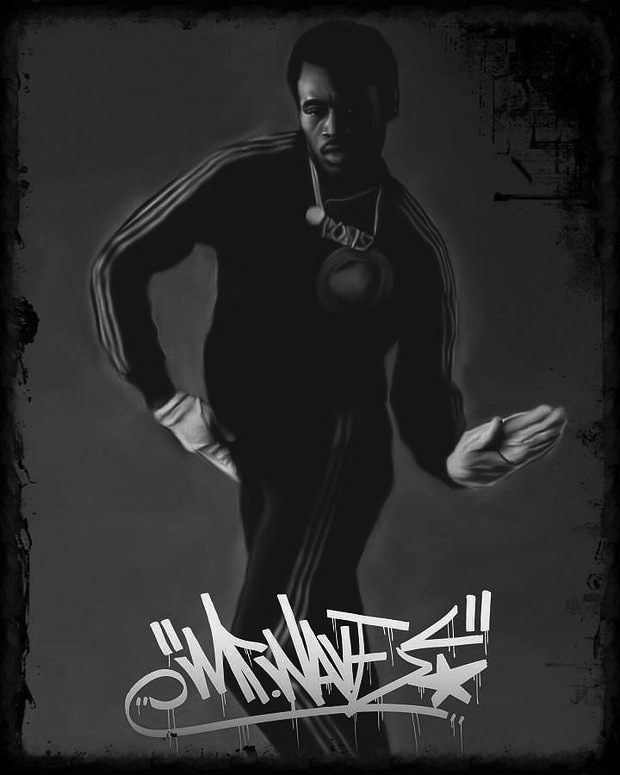
\includegraphics[width=\linewidth]{mr_wave.jpg}
  \caption{Portrait of Mr. Wave}
  \label{fig:marginfig}
\end{marginfigure}

\marginnote[30pt]{Mr. Wave (AKA Tony Draughon) was an original member of New York City Breakers.  As an actor he was best known for his performance in the film classic \textit{Beat Street} (1984).  \\ \ \\ \ \\ \ \\
Waving is an illusionary dance style composed of a series of movements that give the appearance that a wave is traversing through a dancer's body.  Waving is thought to have grown out of the popping and funk dance scene.}

\begin{marginfigure}[60pt]
  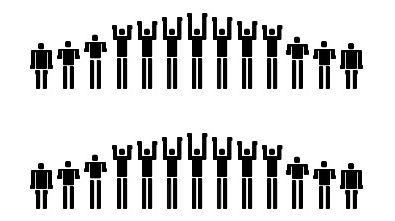
\includegraphics[width=\linewidth]{the_wave.jpg}
  \caption{Diagram of "The Wave"}
  \label{fig:marginfig}
\end{marginfigure}

\section{Media and Disturbance}
\newthought{A wave is a disturbance}, or oscillation, which propagates through space.  It delivers energy, or information, from one point to another.  We begin to theorize waves considering three criteria for their existence.
\begin{itemize}
\item \textbf{source}\\ A disturbance originates from some region of space at some time.
\item \textbf{medium}\\ The disturbance must propagate through some medium. 
\item \textbf{interaction}\\  For the disturbance to propagate through space there must be some physical means by which adjacent portions of the medium interact in order to pass the disturbance through space.
\end{itemize}
This being said, we may imagine a universe where "in the beginning" waves exist and need not a source.  In addition, the vacuum of empty space may provide the medium for energy to propagate.  A medium is typically considered to be an assembly, or continuum, of "stuff" with inertial properties.  Waves may also travel through nothing. 

\section{Wave Types}

\begin{description}
  \item[transverse wave] A propagating wave that causes the particles of the disturbed medium to move \textbf{perpendicular} to the direction of wave propagation.  "The Wave" at sporting events travels through the crowd as a transverse wave.  
  \item[longitudinal wave] A propagating wave that causes the particles of the disturbed medium to move \textbf{parallel} to the direction of wave propagation.  Sound travels through air as a longitudinal wave.
  
\end{description}

\begin{marginfigure}[0pt]
  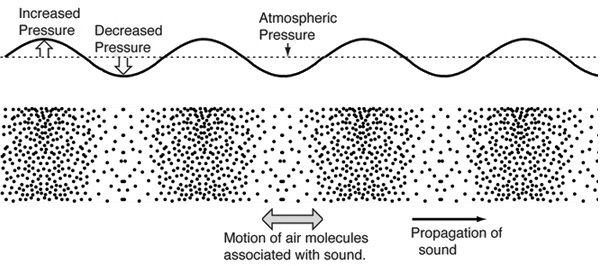
\includegraphics[width=\linewidth]{lwav.jpg}
  \caption{Longitudinal wave}
  \label{fig:marginfig}
\end{marginfigure}

\section {One Dimensional Waves}
A wave can take many forms.  In one dimension a wave can be represented by any function of the position plus/minus the product of velocity and time.  The amplitude $A$ represents the maximum value of the function $f(x \pm vt)$.  The wave velocity is the time rate of change of the position on some point of the function $f(x)$.
$$y=f(x-vt) \hspace{2cm} \text{propagation in positive direction}$$
$$y=f(x+vt) \hspace{2cm} \text{propagation in negative direction}$$
$$A=f_{max}$$
$$v=\lim _{\Delta \rightarrow 0}\frac{\Delta x}{\Delta t}=\frac{dx}{dt}=-\frac{\frac{\partial f}{\partial t}}{\frac{\partial f}{\partial x}}$$

\begin{marginfigure}[-130pt]%
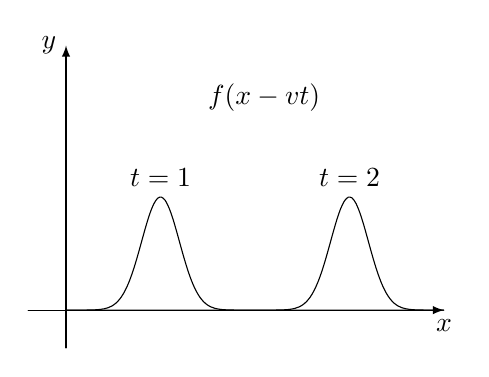
\begin{tikzpicture}
    [line cap=round,line join=round,x=2cm,y=2cm, scale=1.2, decoration={brace,amplitude=2pt}]
 \draw[smooth,samples=100,domain=0:2]
                                 plot(\x,{1.5/(sqrt(2*pi))*exp(-((\x-0.5)^2)/(2*0.1^2))});
 \draw[smooth,samples=100,domain=0:2]
                                 plot(\x,{1.5/(sqrt(2*pi))*exp(-((\x-1.5)^2)/(2*0.1^2))});
   \draw[-latex,color=black,thin] (-0.2,0) -- (2,0) node [anchor=north ,scale=1] {$x$};
   \draw[-latex,color=black,thin] (0,-0.2) -- (0,1.4)node [anchor=east ,scale=1] {$y$};
   \draw (0.7,1) node [anchor=south west ,scale=1] {$f(x-vt)$};
      \draw (0.5,0.6) node [anchor=south ,scale=1] {$t=1$};
   \draw (1.5,0.6) node [anchor=south ,scale=1] {$t=2$};
 \end{tikzpicture}
  \caption{A wave pulse traveling in the positive $x$ direction}
  \label{fig:marginfig}
\end{marginfigure}
 
 \section{Supersposition}
 If two waves are simultaneously propagating through a medium the resultant wave function at any point is the algebraic sum of the wave wave functions of the individual waves.
 
 \section{Waves on Strings (Transverse)}
 \newthought{Consider a wave pulse} traveling along a string with tension $T$ and linear mass density $\mu$.  Zooming in closely to a section of the string the curvature is constant and can therefore be approximated by a circular arc of radius $R$ and angle $\theta$.  \\
The section of string has a net force $F_r$ on it which restores it to equilibrium and a mass $m$.
$$F_r=2F\sin\theta\approx 2F\theta$$
$$m=\mu \Delta s= 2\mu R \theta$$
This force accelerates the section of string centripetally so the velocity of the section of string may be determined as follows.
$$F_r=\frac{mv^2}{R} \hspace{1cm} \longrightarrow \hspace{1cm} 2F\theta=\frac{2\mu R \theta v^2}{R}$$
$$v=\sqrt{\frac{F}{\mu}}$$

\begin{marginfigure}[-220pt]
  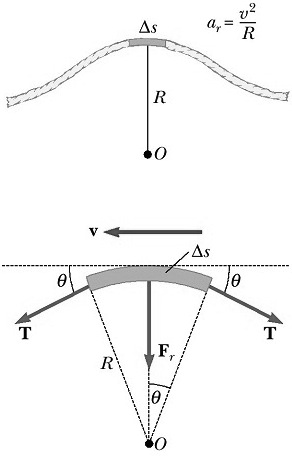
\includegraphics[width=\linewidth]{string_wave.jpg}
  \caption{Transverse wave on a string}
  \label{fig:marginfig}
\end{marginfigure}

 \section{Reflection at an Interface}
 
 \begin{itemize}
\item When a wave meets a free boundary, or travels to a less dense/lower velocity medium,  the reflected pulse is not inverted.
\item When a wave meets a fixed boundary, or travels to a more dense/higher velocity medium, the reflected pulse is inverted. 
\end{itemize}

\begin{marginfigure}[0pt]
  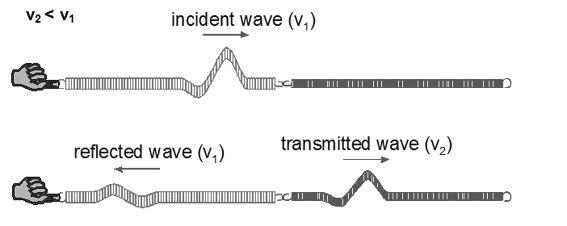
\includegraphics[width=\linewidth]{wave_interface.jpg}
  \caption{Transverse wave at an interface (no inversion)}
  \label{fig:marginfig}
\end{marginfigure}

\begin{marginfigure}[0pt]
  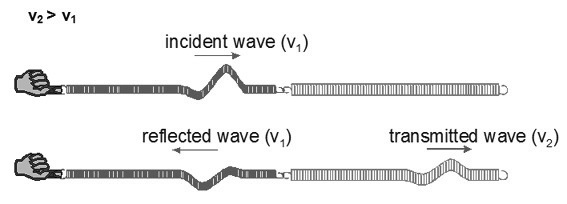
\includegraphics[width=\linewidth]{wave_interface2.jpg}
  \caption{Transverse wave at an interface (inversion)}
  \label{fig:marginfig}
\end{marginfigure}

\section{Sinusoidal Waves}
A sinusoidal wave is the smoothest periodic wave.  Here $y$ represents the displacement from equilibrium.  It can represent pressure or a spatial dimension.  $A$ is the amplitude.  It is the maximum $y$ value.  $x$ is the spatial dimension in the direction of propagation.  $t$ is time.  $\phi$ is the phase.  $k$ and $\omega$ are the coefficients of $x$ and $t$ respectively.  
$$y=A\cos\left( kx - \omega t+\phi\right)$$
$k$ and $\omega$ determine the spatial and temporal periodicity.  $\lambda$ is the wavelength and $T$ is referred to as the period.  The wave length is the distance between identical points in the wave.  The period is the time between wave cycles.
$$k\lambda=2\pi \hspace{2cm} \omega T=2\pi$$
The wave speed is defined as the ratio of the wavelength and the period.  It is the speed at which some point on the pattern travels.  It does not represent the speed of any particles in the medium.
$$v_{wave}=\frac{\lambda}{T}=\frac{\omega}{k}$$

\begin{figure}
  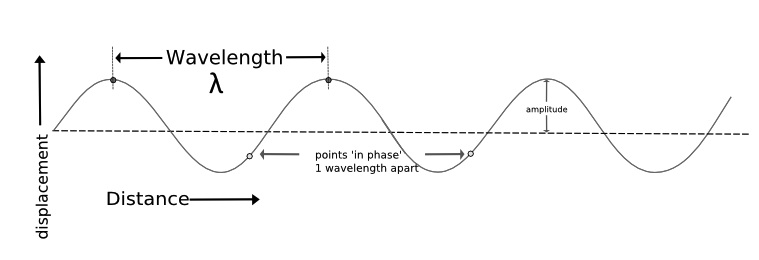
\includegraphics[width=\linewidth]{sine_wave.jpg}
  \caption{Sine wave }
  \label{fig:marginfig}
\end{figure}

\subsection{Power}
\marginnote{The power delivered by the wave can be thought of as the rate kinetic energy is delivered in the medium. }
$$\Delta E=\frac{1}{2}(\Delta m)\omega^2A^2=\frac{1}{2}(\mu \Delta x)\omega^2A^2$$
$$P=\frac{\Delta E}{\Delta t}=\frac{1}{2}\mu\omega^2A^2 \frac{\Delta x}{\Delta t}=\frac{1}{2}\mu\omega^2A^2 v_{wave}$$

\newpage

\section{Wave Equation}
Given a scalar function $u(\overrightarrow{\scriptr})$, such as pressure, and propagation speed $c$ we have the following differential equation.  This is known as the wave equation. 
$${\partial^2 u \over \partial t^2} = c^2 \nabla^2 u$$
The functions which obey this differential relationship are waves.  When this differential equation arrises in the analysis of some system it means the systems supports the propagation of waves.

\marginnote{The speed of sound varies with temperature, pressure and the density of the material.  The speed of sound (m/s) in air (at 1 atm) varies with temperature (Celsius) as follows.
$$v=331+0.6T$$}
\section{Sound Waves}
Sound is defined by ANSI as "Oscillation in pressure, stress, particle displacement, particle velocity, etc., propagated in a medium with internal forces (elastic or viscous)."  It can propagate through compressible media such as air, water and solids as longitudinal waves or transverse waves in solids. 
\marginnote{Humans can hear sounds in the range of 20 to 20,000 Hertz, though there is variation between individuals.  Elephants can hear sounds at 14-16hz, while some whales can hear subsonic sounds as low as 7hz (in water).}


The velocity of sound in a medium depends its elastic and inertial properties.
$$v=\sqrt{\frac{\text{elastic property}}{\text{inertial property}}}=\sqrt{\frac{B}{\rho}}$$
\subsection{Power, Intensity and Sound Level}
Consider a sound source emitting energy at a rate $P$.  This is the power of the source.  The intensity of the sound, captured by some observer, is the power per unit area.
$$I=\frac{\text{Power}}{\text{Area}}$$
\begin{marginfigure}[0pt]
  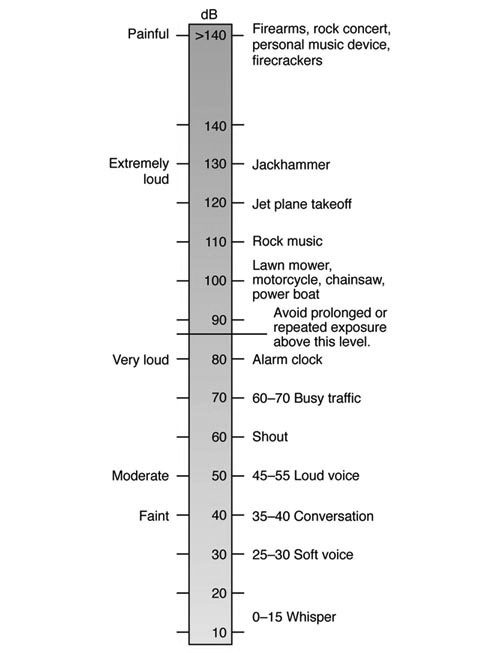
\includegraphics[width=\linewidth]{decibel.jpeg}
  \caption{The decibel scale}
  \label{fig:marginfig}
\end{marginfigure}
The decibel scale of intensity is a logarithmic scale.  The reference value $I_0$ is the lowest intensity of audible sound.
$$\beta=10\  \log \frac{I}{I_0} \hspace{2cm} I_0=10^{-12} \ W/m^2$$

\subsubsection{Spherical, Cylindrical and Linear Waves}
Spherically symmetric waves disperse power over the the surface of a sphere.  Cylindrically symmetric waves disperse power over the the surface of a cylinder.
$$I_{sphere}=\frac{P}{4\pi r^2} \hspace{2cm} I_{cyl}=\frac{P}{2\pi r}$$
Symmetric waves in one dimension give the following intensity.
$$I=\frac{P}{2}$$


\subsection{Doppler Effect}
The Doppler effect is the change in frequency of a wave for an observer moving relative to its source. It is named after the Austrian physicist Christian Doppler, who proposed it in 1842 in Prague. It is commonly heard when a vehicle sounding a siren or horn approaches, passes, and recedes from an observer. Compared to the emitted frequency, the received frequency is higher during the approach, identical at the instant of passing by, and lower during the recession.

$$f = \left ( \frac {c+v_\text{reciever}}{c + v_\text{source}} \right ) f_0$$
\subsection{Standing Waves \& Resonance}
A standing wave is associated with each point on the axis of the wave having an associated constant amplitude. The locations at which the amplitude is minimum are called nodes, and the locations where the amplitude is maximum are called antinodes.

It arises as a result of interference between two waves traveling in opposite directions.  Resonance is the manifestation of standing waves inside a resonator due to interference between waves reflected back and forth at the resonant frequency.
\marginnote{
$$\cos{a}+\cos{b}=2\cos\frac{a+b}{2}\cos\frac{a-b}{2}$$ 
\\ \ \\
$$\sin{a}\pm\sin{b}=2\sin\frac{a\pm b}{2}\cos\frac{a\mp b}{2}$$}

$$A_0\cos(kx-\omega t)+A_0\cos(kx+\omega t)=2A_0 \cos(kx)\cos(\omega t)$$

\subsection{Beats}
A beat is an interference pattern between two sounds of slightly different frequencies, perceived as a periodic variation in volume whose rate is the difference of the two frequencies.  When tuning instruments that can produce sustained tones, beats can readily be recognized. 
$$A_0\cos(\omega_1 t)+A_0\cos(\omega_2 t)=2A_0 \cos(\frac{\omega_1-\omega_2}{2}t)\cos(\frac{\omega_1+\omega_2}{2}t)$$
%\chapter{Electrostatics}

\textit{We call that fire of the black thunder-cloud 'electricity,' and lecture learnedly about it... but what is it?}\\
\noindent\textbf{-   Thomas Carlyle}

\vspace{1cm}


\begin{marginfigure}%
  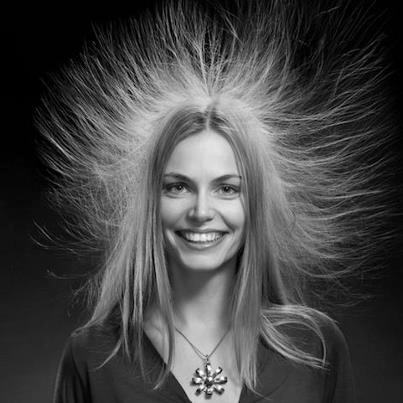
\includegraphics[width=\linewidth]{hair_static.jpg}
  \caption{Amber and her charged hair}
  \label{fig:marginfig}
\end{marginfigure}

\marginnote{In the colder months, when the air has less moisture, hair picks up electrical charge.  Fight this unfortunate situation by switching to a more hydrating shampoo and conditioner.}

\section{Background}
Electrostatics deals with the phenomena and properties of stationary charges.   The ancients knew materials such as amber attract lightweight particles after rubbing.   Thales of Miletus made a series of observations on static electricity around 600 BC.  The word electricity comes from the Greek word for amber.  Electrostatic phenomena arise from the forces that electric charges exert on each other.
\begin{itemize}
\item there are two kinds of charge in nature of which opposite attract and like repel
\item charge is conserved
\item charge is quantized
\end{itemize}

\section {Coulomb's Law}

\begin{marginfigure}%
  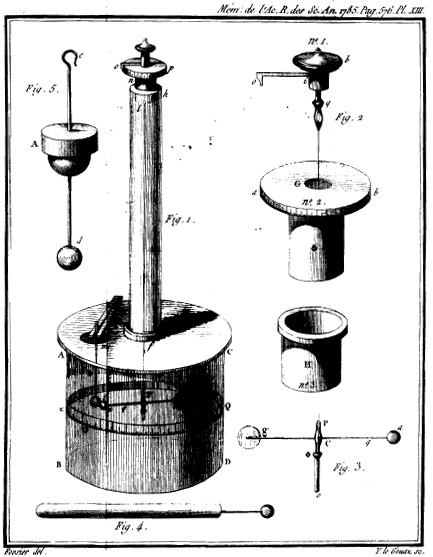
\includegraphics[width=\linewidth]{torsion.jpg}
  \caption{Coulomb's torsion balance}
  \label{fig:marginfig}
\end{marginfigure}

Coulomb's law describes the electrostatic interaction between electrically charged particles. The law was first published in 1784 by French physicist Charles Augustin de Coulomb. It is analogous to Isaac Newton's inverse-square law of universal gravitation.

$$F_{E}=k_e\frac{q_1q_2}{r^2}$$
$$\overrightarrow{F}_{2\rightarrow 1}=-k_e\frac{q_1q_2}{r^2} \hat{r} \hspace{2cm} \overrightarrow{r}=\overrightarrow{r}_2-\overrightarrow{r}_1$$


$$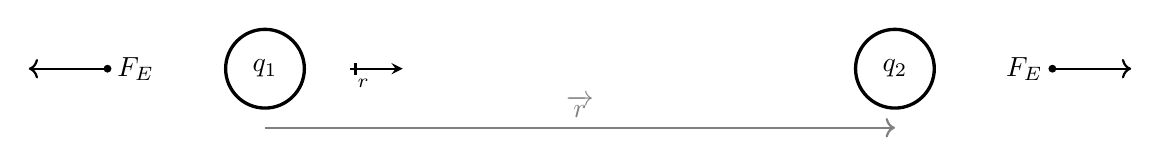
\begin{tikzpicture}[scale=1]
     	
	\fill[black] (-6,0) circle (0.5mm) node [anchor=west ,scale=1] {$F_E$};   
	\draw[->,thick] (-6,0) -- (-7,0) ; 
	\fill[black] (6,0) circle (0.5mm) node [anchor=east,scale=1] {$F_E$};   
	\draw[->,thick] (6,0) -- (7,0) ; 
	 \draw[very thick] (-4,0) circle (0.5cm) node {$q_1$};
	  \draw[very thick] (4,0) circle (0.5cm) node {$q_2$};
	    \draw[thick, color=gray,->] (-4,-0.75) --   (4,-0.75) node [midway, anchor=south] {$\overrightarrow{r}$};
	     
	     
	       \begin{scope}[shift={(-3,0)}, scale=0.75] 
	 
	   \draw[thick](0.2,0.1) -- (0.2,-0.1);
	    \draw[ thick,-stealth] (0.1,0) -- (1,0) node [near start,anchor=north]{\scriptsize $r$};  
	  \end{scope}	     
   \end{tikzpicture}$$


\newpage

\section{Constants}

\begin{table}[h]\index{typefaces!sizes}
  \footnotesize%
  \begin{center}
    \begin{tabular}{lcl}
      \toprule
     Constant & Variable & Quantity \\
      \midrule
 Electrostatic Constant   & $k_e$           & $8.9875 \times 10^{9}\  \nicefrac{ \text{N}\cdot\text{m}^2}{\text{C}^2}$    \\
    Fundamental Charge       & $e$             & $1.6022 \times 10^{-19}\  \text{C}$                                          \\
    Mass of the Electron     & $m_e$           & $9.1095 \times 10^{-31}\  \text{kg}$                                         \\
    Mass of Proton           & $m_p$           & $1.6726 \times 10^{-27} \ \text{kg}$                                         \\ 
    Mass of Neutron           & $m_n$           & $1.6749 \times 10^{-27}\  \text{kg}$                                         \\ 
    Vacuum Permativity       & $\epsilon_0$ & $8.8542 \times 10^{-12}\  \nicefrac{ \text{F}}{\text{m}}$                    \\ 
    Speed of Light       & $c$ & $2.998 \times 10^{8}\  \nicefrac{ \text{m}}{\text{s}}$                    \\ 
      \bottomrule
    \end{tabular}
  \end{center}
  \caption{Physical constants for electrostatics}
  \label{tab:font-sizes}
\end{table}

\marginnote[-50pt]{
$$ k_e=\frac{1}{4\pi \epsilon_0}$$}


\marginnote[0pt]{
The unit of electric charge is the Coulomb, denoted C.}

\section {Electric Field}
The concept of an electric field, or E-field, was introduced by Michael Faraday.  The electric field $\overrightarrow{E}(\overrightarrow{r})$ is a vector field, meaning it is a vector quantity at every point in space.  At a single point in space, the electric field represents the force that would be exerted on a one Coulomb "test charge".  The E-field is the electrostatic force per unit charge.
$$\overrightarrow{E}=\frac{\overrightarrow{F}_e}{q_0}$$
There is an electric field surrounding every charge distribution.  Consider the E-field to represent a feature of space that represents the possibility of electric force, if there were a charge there.
\subsection{Point Charge}
Consider a point charge located at point $\overrightarrow{b}$.  The electric field at a location $\overrightarrow{r}$, due to the presence of the  point charge is represented as follows.  
$$\overrightarrow{E}(\overrightarrow{r})=k_e\frac{q}{R^2}\hat{R} \hspace{1cm} \overrightarrow{R}=\overrightarrow{r}-\overrightarrow{b}$$
A point charge located at the origin of coordinates will generate the following electric field
$$\overrightarrow{E}(\overrightarrow{r})=k_e\frac{q}{r^2} \hat{r} $$

\marginnote[-300pt]{
\subsection{Superposition}
The principle of superposition applied to electrostatic distributions means the force on a given charge $Q$ is the vector sum of forces from interactions with a set of charges.  
$$\overrightarrow{F}_E=k_e\sum_{i=1}^{N} \frac{Qq_i}{R_i^2} \hat{R}_i $$
Equivalently the electric field at a given point in space is the vector sum of the fields due to the set of charges around it.
$$\overrightarrow{E}(\overrightarrow{r})=k_e\sum_{i=1}^{N} \frac{q_i}{R_i^2} \hat{R}_i $$
}


\begin{marginfigure}[-60pt]%
  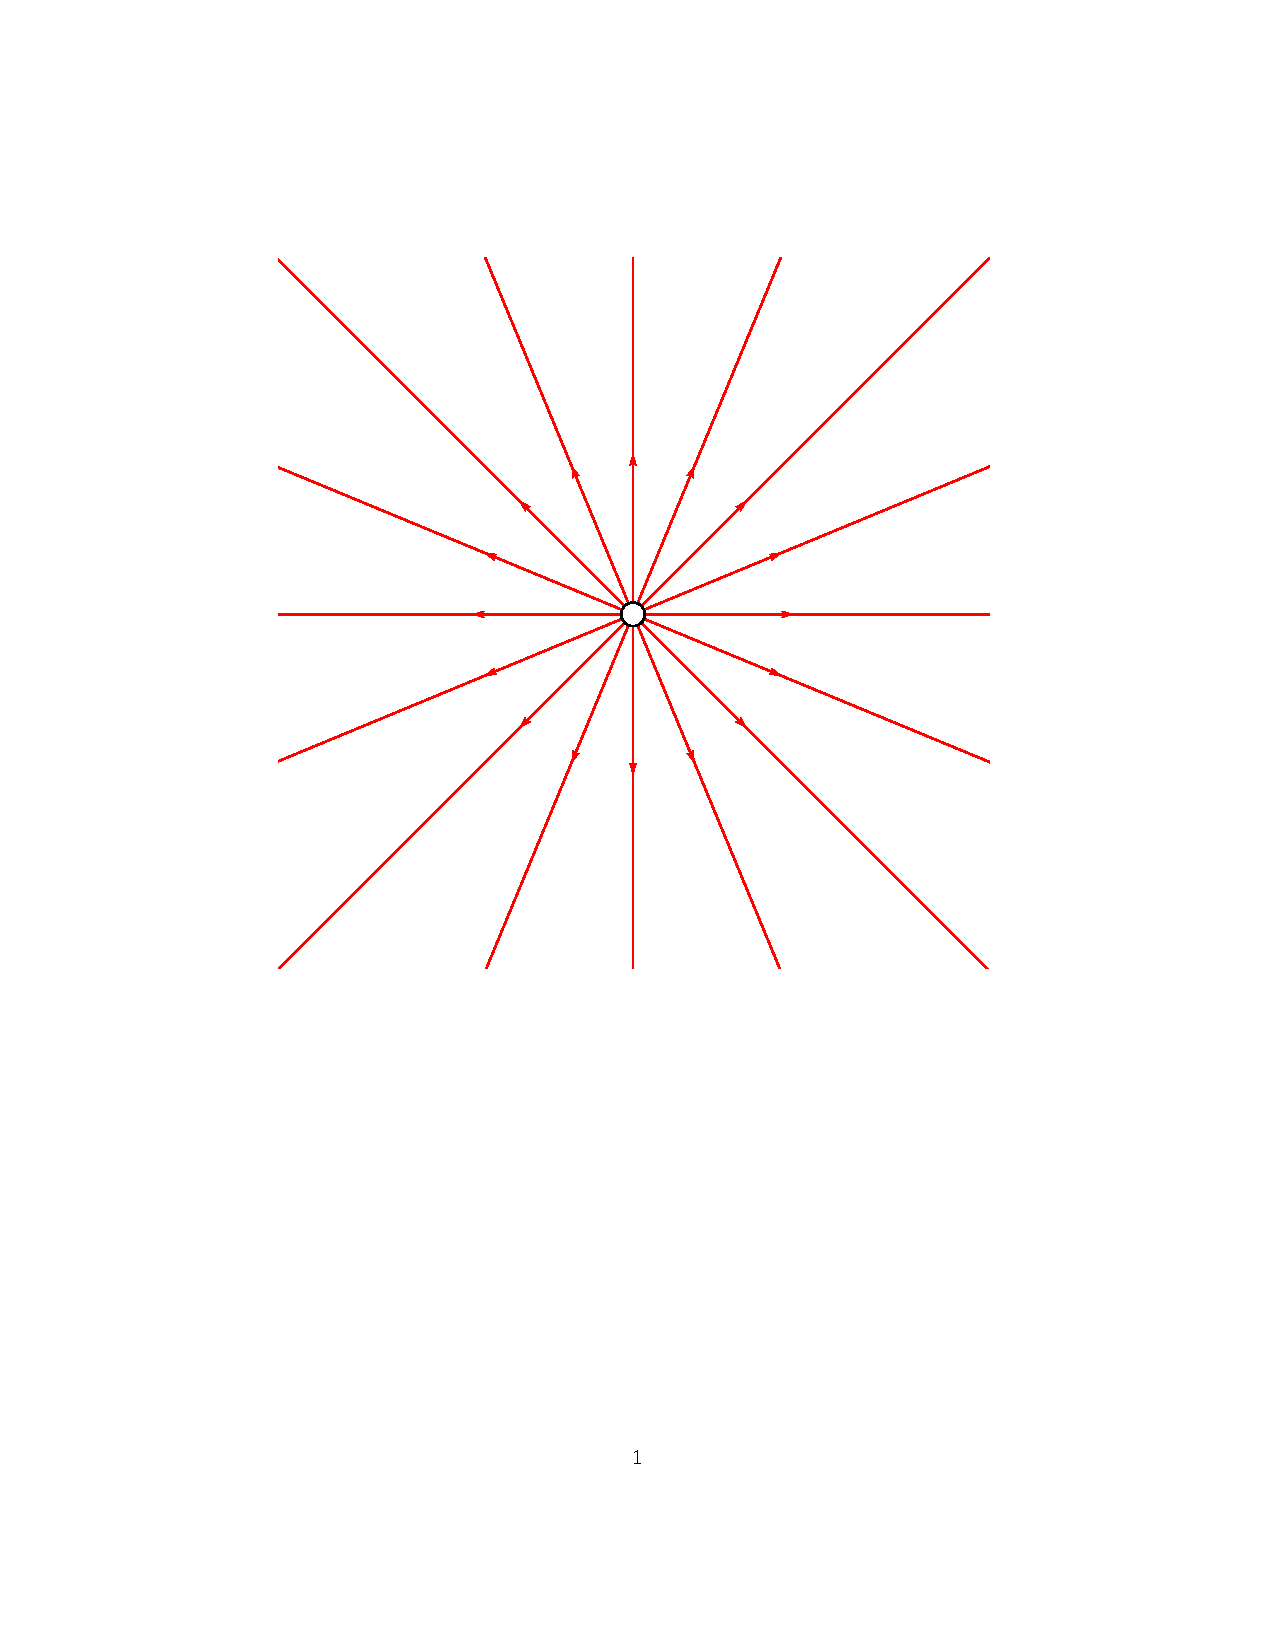
\includegraphics[width=\linewidth ,trim={7cm 14cm 7cm 7cm},clip]{monopole_graph.pdf}
  \caption{Single positive charge}
  \label{fig:marginfig}
\end{marginfigure}




  \section{Electric Field Lines}
  Electric field lines are a visual tool used to visualize the strength and direction of the electric field in space.  While they are not real, per se, they provide an extremely useful representation for the permeation of electric field through space.  
  \begin{itemize}
 \item Electric field lines emanate perpendicularly out of positive charge and sink perpendicularly into negative charge.  They may also terminate/emanate at infinity if the net charge of the distribution is non-zero.
 \item The number of field lines drawn entering/exiting a charge is proportional to the amount (magnitude) of charge.
 \item  The electric field vector is directed tangent to the field line at each point in space.
 \item No two field lines can cross
 \item  The number of lines per unit area is proportional to the field strength in that area.  Thus $E$ is strong when field lines are close together while $E$ is weak when field lines are far apart.
 \
 \end{itemize}


\begin{marginfigure}[-250pt]%
  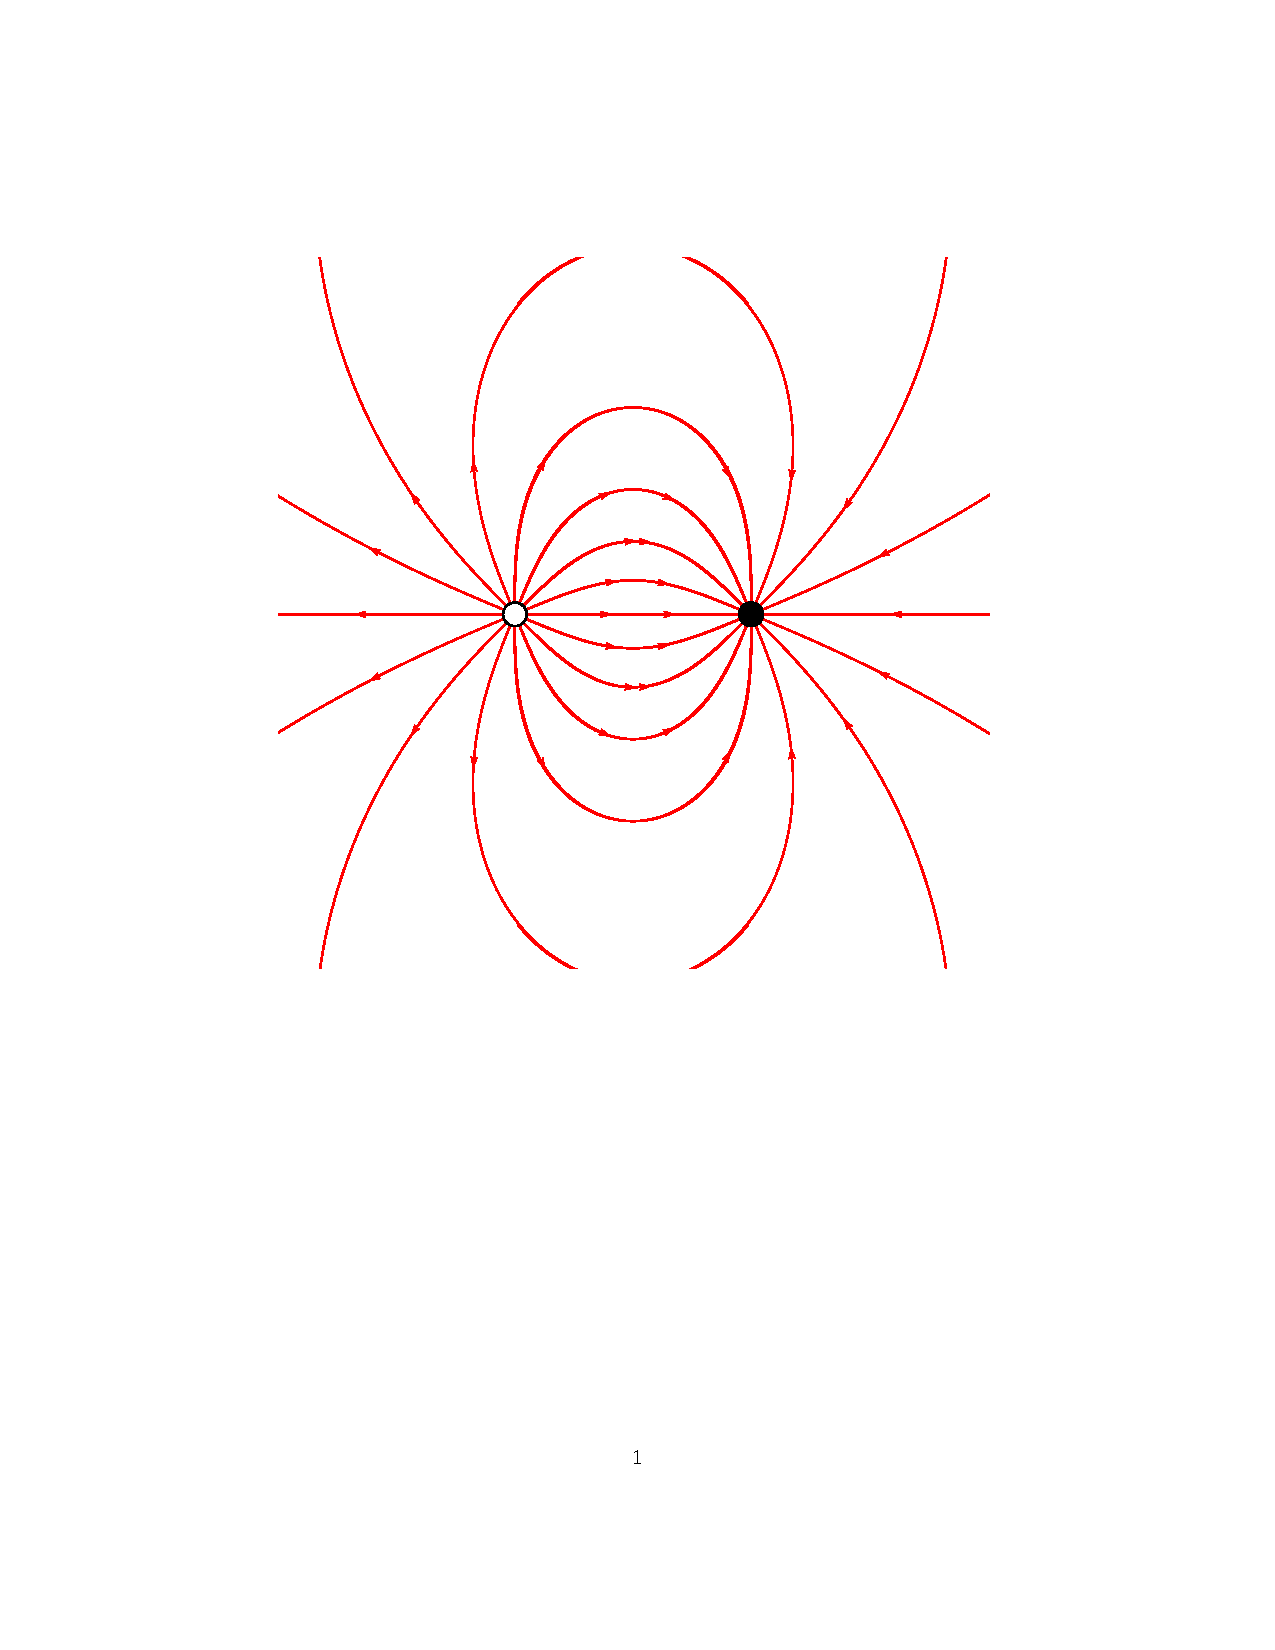
\includegraphics[width=\linewidth ,trim={7cm 14cm 7cm 7cm},clip]{dipole_graph.pdf}
  \caption{Dipole field close up}
  \label{fig:marginfig}
\end{marginfigure}

\begin{marginfigure}[-40pt]%
  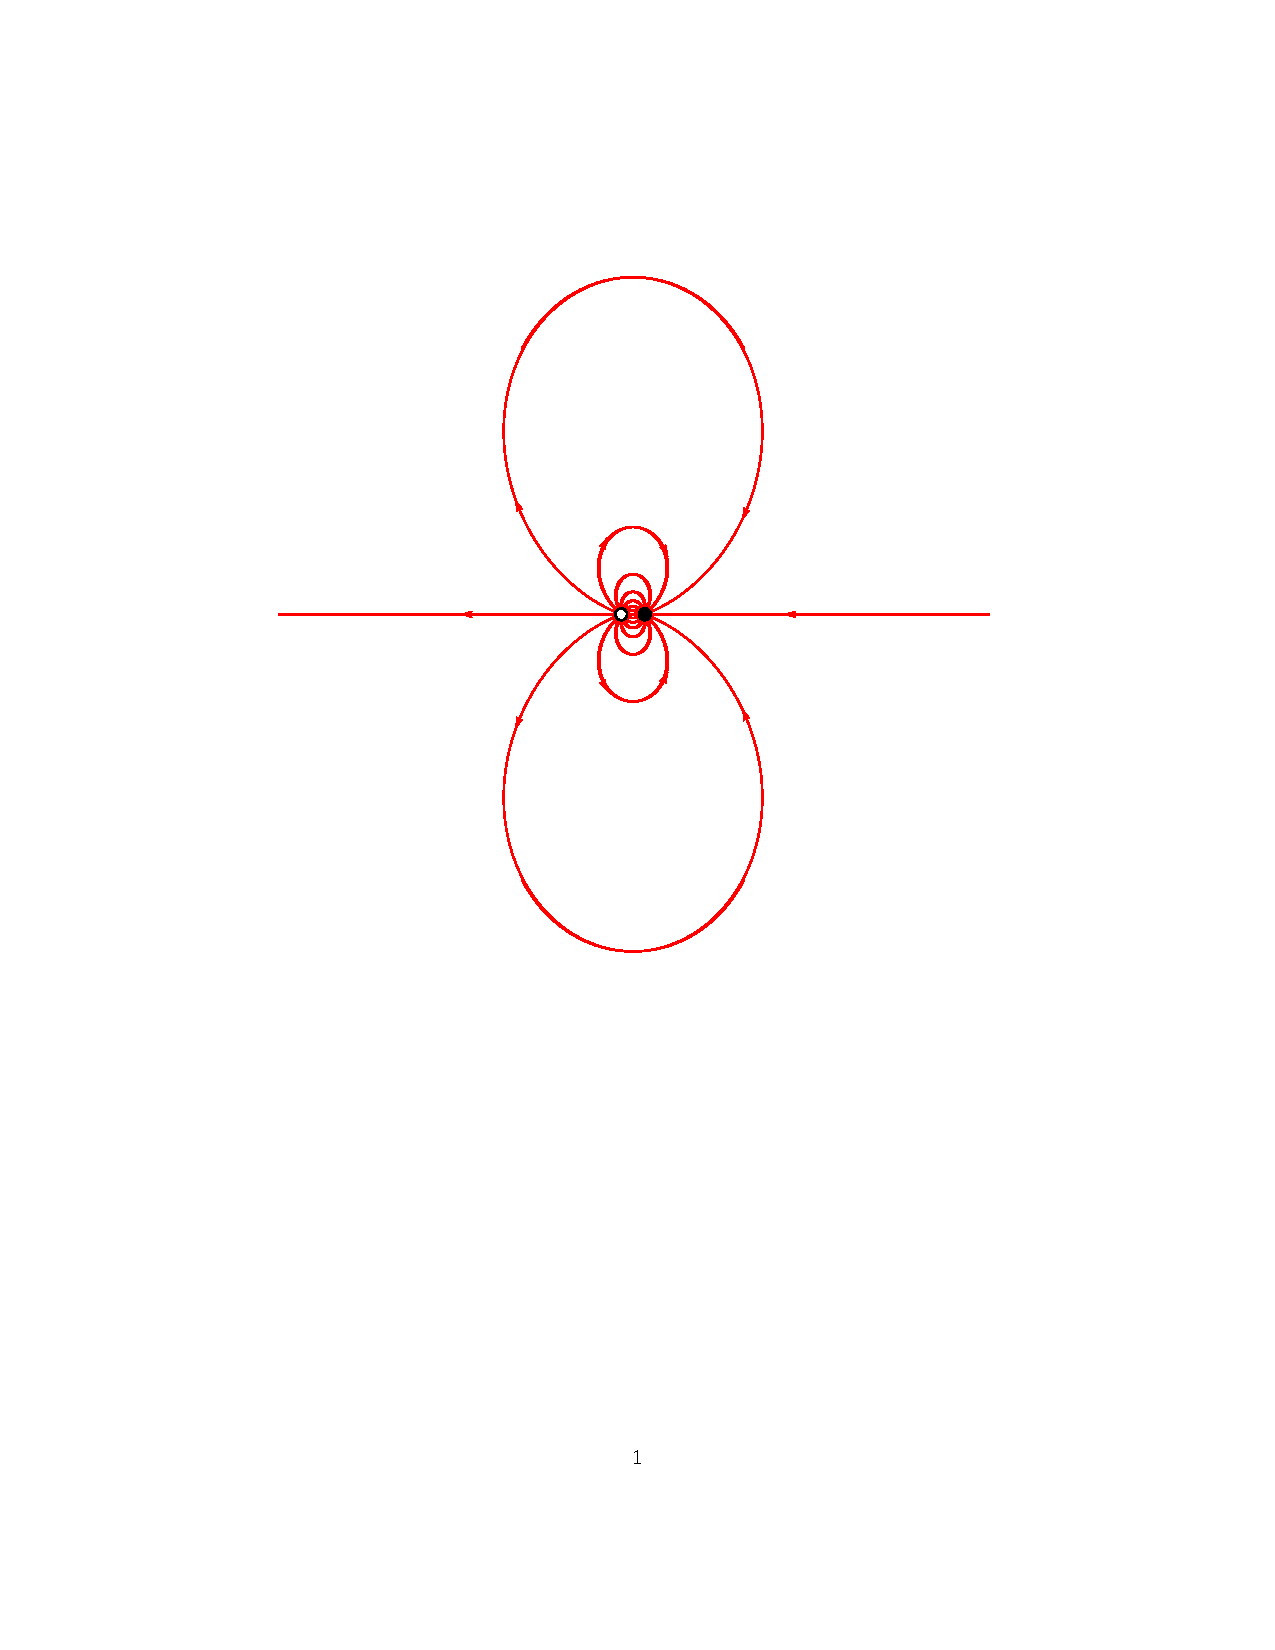
\includegraphics[width=\linewidth ,trim={7cm 15cm 7cm 8cm},clip]{dipole_far2.pdf}
  \caption{Dipole field far away}
  \label{fig:marginfig}
\end{marginfigure}

\begin{marginfigure}[10pt]%
  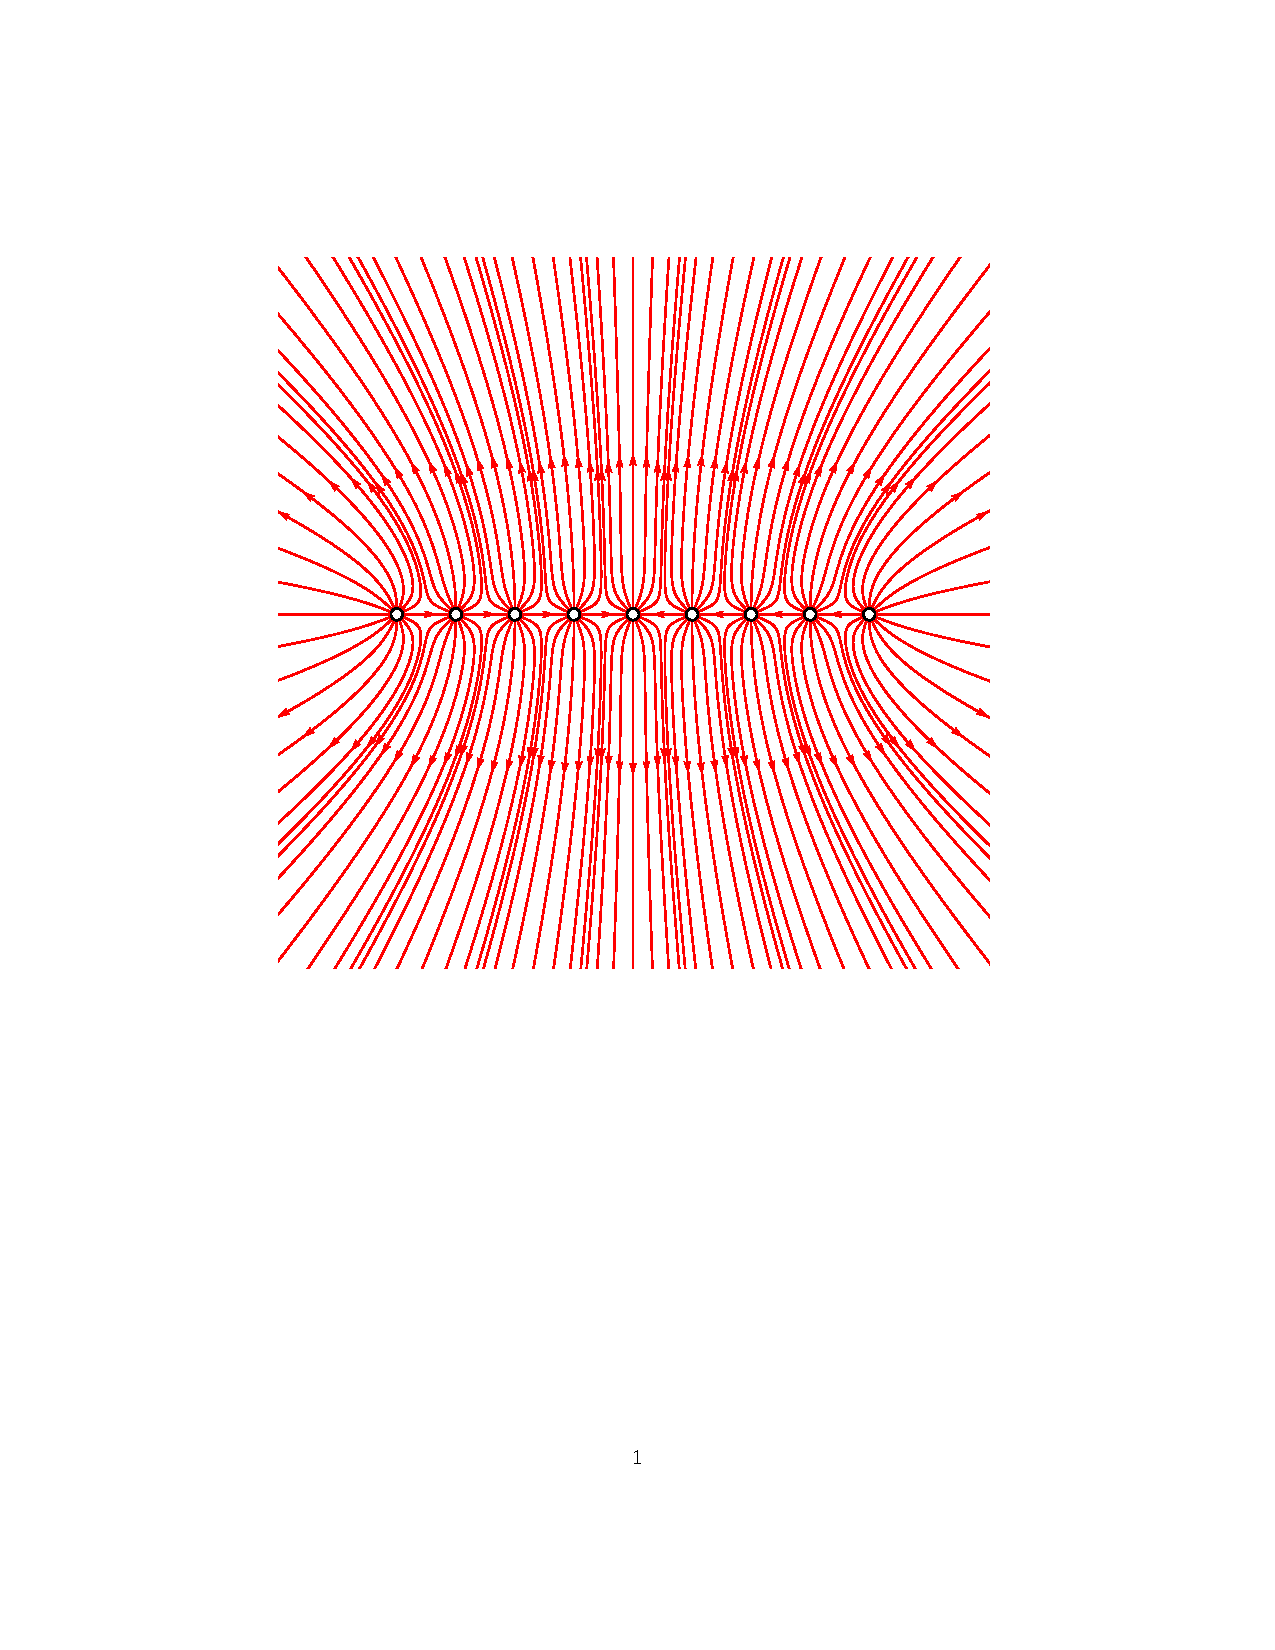
\includegraphics[width=\linewidth ,trim={6cm 14cm 6cm 7cm},clip]{Efield_graph2.pdf}
  \caption{Superposition of multiple positive point charges in a row}
  \label{fig:marginfig}
\end{marginfigure}

\begin{marginfigure}[0pt]%
  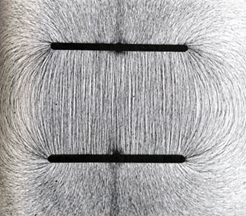
\includegraphics[width=\linewidth]{electric_fields.jpg}
  \caption{Electric field between two charged plates}
  \label{fig:marginfig}
\end{marginfigure}

%\subsection{Continuous Distribution}
%$$\overrightarrow{E}=k_e\int \frac{dq}{r^2} \hat{r} $$

 
 \section{Charge Distributions}
 A charge distribution is any arrangement of charge in space.  It may consist of a set of various point charges at different locations in space or be a continuous distribution of charge.  Continuous charge distributions may be represented by charge per unit volume, charge per unit area, or charge per unit distance.  These are  types of charge density. 
 $$\text{Volume density} \hspace{2cm} \rho=\frac{Q}{V}$$
  $$\text{Surface density} \hspace{2cm} \sigma=\frac{Q}{A}$$
   $$\text{Line density} \hspace{2cm} \lambda=\frac{Q}{L}$$
   
 \section{Types of Materials}
Atomic lattices making up bulk materials have different electron energy levels or bands.  \textbf{Valence bands} are associated with individual atomic orbital.  Their electrons are spatially localized and lower energy.   \textbf{Conduction bands} are associated with delocalized or free electrons able to move throughout the bulk material.  The energy difference between the highest valence band and lowest conduction band is known as the \textbf{band gap}.  Electrons fill lowest first.  The \textbf{Fermi level} is a thermodynamic property that corresponds to the hypothetical energy of an electron added to the system.  
   
 \newpage  
   
 \begin{description}
  \item[Conductors] In conductors the Fermi level is in conduction band.  This means electrons added to the system are not spatially isolated and is free to move around.  This so called "free charge" accumulates on the surface of the bulk material and congregates more densely in kinks and furrows.
  \item[Insulators]  For insulators the Fermi level in a large band gap.  There are no free electrons.  They are bound locally.  Charge is not free to move around.
   \item[Semiconductors]  In semiconductors the band gap is small so electrons can be easily bumped from localized states to delocalized states in conduction bands.
\end{description}
  
   
   \begin{marginfigure}[-180pt]%
  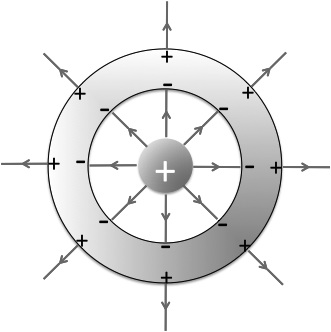
\includegraphics[width=\linewidth]{conductor.jpg}
  \caption{Electric field and charge distribution in a conducting sphere}
  \label{fig:marginfig}
\end{marginfigure}

\begin{marginfigure}[40pt]%
  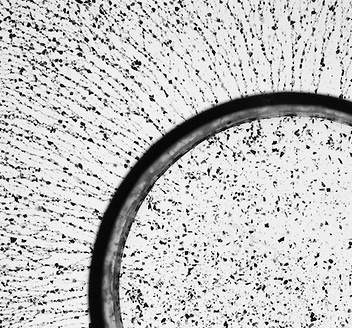
\includegraphics[width=\linewidth]{conductor2.jpg}
  \caption{Electric field inside and outside a conducting sphere}
  \label{fig:marginfig}
\end{marginfigure}
   
 \section{Field and Charge Distributions in Conductors}
 \begin{itemize}
 \item The electric field is zero everywhere inside the conductor.
 \item  Any charge on an isolated conductor resides on its surface.
 \item  The electric field just outside a charged conductor is perpendicular to the surface and has a magnitude of $\frac{\sigma}{2\epsilon_0}$.
 \item On an irregularly shaped conductor, charge tends to accumulate at locations where the radius of curvature is smallest such as edges, corners and points.
 \end{itemize}
 

\begin{marginfigure}[80pt]%
  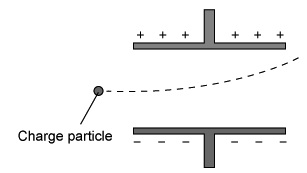
\includegraphics[width=\linewidth]{charge_particle.jpg}
  \caption{Motion of charged particle between two charged plates}
  \label{fig:marginfig}
\end{marginfigure}

 \section{Motion of a Charged Particle}
 Electromagnetic forces are similar to gravity in their relationship to space but are extremely different in one respect.  In gravity mass is responsible for gravitational force but also provides inertia.  For charged particles charge is the source of the electrostatic force but mass still provides the inertia.  
 $$\overrightarrow{F}_{net}=m\overrightarrow{a}$$
 $$\overrightarrow{F}_{net}=q\overrightarrow{E} \hspace{1cm} \longrightarrow \hspace{1cm} \overrightarrow{a}=\frac{q}{m}\overrightarrow{E}$$
 If we generate a field in space and drop a particle in that field then the charge-to-mass ratio can be known through measuring the acceleration.

\newpage

\begin{marginfigure}[50pt]%
  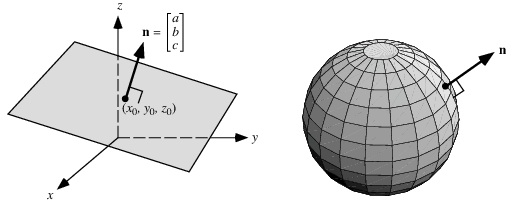
\includegraphics[width=\linewidth]{normal.jpg}
  \caption{Surface normal vector}
  \label{fig:marginfig}
\end{marginfigure}

\begin{marginfigure}[0pt]%
  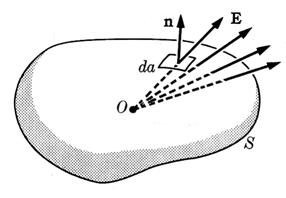
\includegraphics[width=\linewidth]{gauss_law.jpg}
  \caption{Schematic of Gauss's law }
  \label{fig:marginfig}
\end{marginfigure}

  \section{Electric Flux}
  Electric flux, $\Phi_E$, is the measure electric field passing through a given surface area. Electric flux is proportional to the number of electric field lines perforating the surface.  
  \subsection{Uniform Field Through a Flat Surface}
  For a flat surface and constant field it is the dot product of the electric field vector and the vector normal to the surface.  A surface normal vector points straight out of a surface.
  $$\Phi_E=EA\cos\theta=\overrightarrow{E}\cdot \overrightarrow{A}$$  
  \subsection{Variable Field Through a Set of Flat Surfaces}
  For a variable field through a set of flat surfaces simply take the sum of the flux through all of the surfaces.
  $$\Phi_E=\sum_{i=1}^{N} \overrightarrow{E}_i\cdot \overrightarrow{A}_i$$
   \subsection{Variable Field Through a Continuous Surface}
   A variable field through a continuous smoothly curved surface is modeled as the limit of area elements going to zero. 
   $$\Phi_E=\lim_{\Delta A \rightarrow 0 }\sum_{i=1}^{N} \overrightarrow{E}_i\cdot \Delta \overrightarrow{A}_i$$
   
   \marginnote[-100pt]{
    $$\lim_{\Delta A \rightarrow 0 }\sum_{i=1}^{N} \overrightarrow{E}_i\cdot \Delta \overrightarrow{A}_i=\lim_{\Delta V \rightarrow 0 }\sum_{j=1}^{M} \nabla \cdot \overrightarrow{E}_i\Delta {V}_i$$
}

 \marginnote[-50pt]{
    $$q_{enc}=\lim_{\Delta V \rightarrow 0 }\sum_{j=1}^{M} {\rho}_i\Delta {V}_i$$
}

   \marginnote{
    $$ \nabla \cdot \overrightarrow{E}_i=\frac{ {\rho}_i}{\epsilon_0}$$
}
     \section{Gauss's Law}
     Gauss's law states the total of the electric flux out of a closed surface is equal to the charge enclosed divided by the permittivity.
    \subsection{Variable Field Through a Continuous Closed Surface}
    $$\Phi_E=\lim_{\Delta A \rightarrow 0 }\sum_{i=1}^{N} \overrightarrow{E}_i\cdot \Delta \overrightarrow{A}_i=\frac{q_{inc}}{\epsilon_0}$$
     \subsection{Uniformly Normal Field of Constant Magnitude Through a Continuous Closed Surface}
     $$\Phi_E=EA=\frac{q_{inc}}{\epsilon_0}$$
     
 

 \begin{marginfigure}[-100pt]%
 $$ 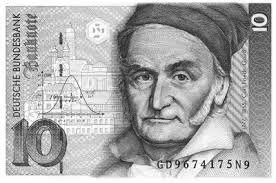
\includegraphics[width=\linewidth]{gauss_money.jpeg}$$
  \caption{Gauss on money }
  \label{fig:marginfig}
\end{marginfigure}

    \newpage

  \section{Work and Electrostatic Potential Energy}
   
  \marginnote[0pt]{The potential energy $U$ is undetermined up to a constant.  The real physically measurable quantity is the change in potential energy, $\Delta U$.}
  
  \marginnote[10pt]{An individual particle does not have potential energy, $U$ resides in the field (if anywhere) and "belongs" to the system as a whole.  If two charged particles are in proximity they do not each have a potential energy.  There is one electrostatic potential energy between the two particles.}
  
  \marginnote[10pt]{Potential energy is only a meaningful concept for certain types of forces, namely conservative forces.  Remember, the total work done on a particle moving from point $A$ to point $B$ must be independent of path for conservative forces.  }
  
  Electrostatic potential energy, $U$, that results from Coulomb forces and is associated with the configuration of a particular set of point charges within a defined system.  An object contributes to the electrostatic potential energy of a system due to its own electric charge and its relative position to other electrically charged objects.
 
  Recall the definition for change in potential energy and the definition of work.
  $$\Delta U=-W \hspace{1cm} W= \sum_A^B \overrightarrow{F}\cdot \Delta\overrightarrow{s}$$
  Combining the above, and expressing the force in terms of the field, yields the following equation.
  $$\Delta U =- q_0 \sum_A^B \overrightarrow{E}\cdot \Delta\overrightarrow{s}$$
  Consider path-summation on the right hand side of the equation.  Note it is purely a function space, the field in the space and the path.  It is independent of the charge.  In addition, since the electrostatic force is conservative, this path-summation is path-independent.   Therefore it only depends on the endpoints of the path and not the path itself.
  
  \section{Electric Potential}
   \marginnote[0pt]{$$\text{Volt}\equiv\frac{\text{Joule}}{\text{Coulomb}}$$}
    \marginnote[0pt]{ }
  We name the field path-summation $\Delta V$, the change in electric potential.
  $$\Delta V=-\sum_A^B \overrightarrow{E}\cdot \Delta \overrightarrow{s}$$
  $\Delta V$ can be considered the change in electrostatic potential energy per unit charge.
  $$\Delta V=\frac{\Delta U}{q_0}$$
  Finally, after choosing a zero reference, we can write the equation representing the voltage (electric potential) as the electric potential energy per unit charge.
  $$V(\overrightarrow{r})=\frac{U(\overrightarrow{r})}{q_0}$$
   \begin{marginfigure}[0pt]%
 $$ 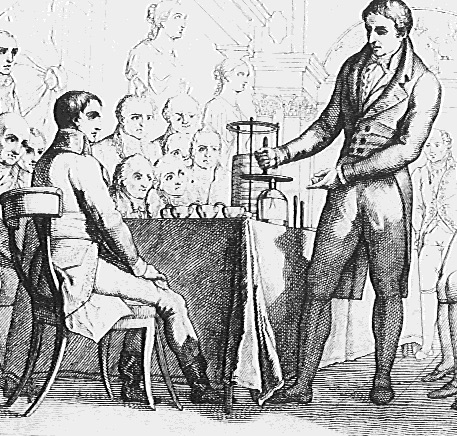
\includegraphics[width=\linewidth]{volt.jpg}$$
  \caption{Alessandro Giuseppe Antonio Anastasio Volta showing his experiments in electricity to Napolean Bonaparte}
  \label{fig:marginfig}
\end{marginfigure}
  The electric potential is a scalar field.  Like the electric field, it is a feature of space independent of the charge we put in the space.  While the electric field represents a vector quantity at every point in space, the voltage (electric potential) represents a single value quantity (scalar quantity) at every point in space.
  
  \newpage
  
  \subsection{Uniform Field}
  \begin{marginfigure}[-10pt]%
  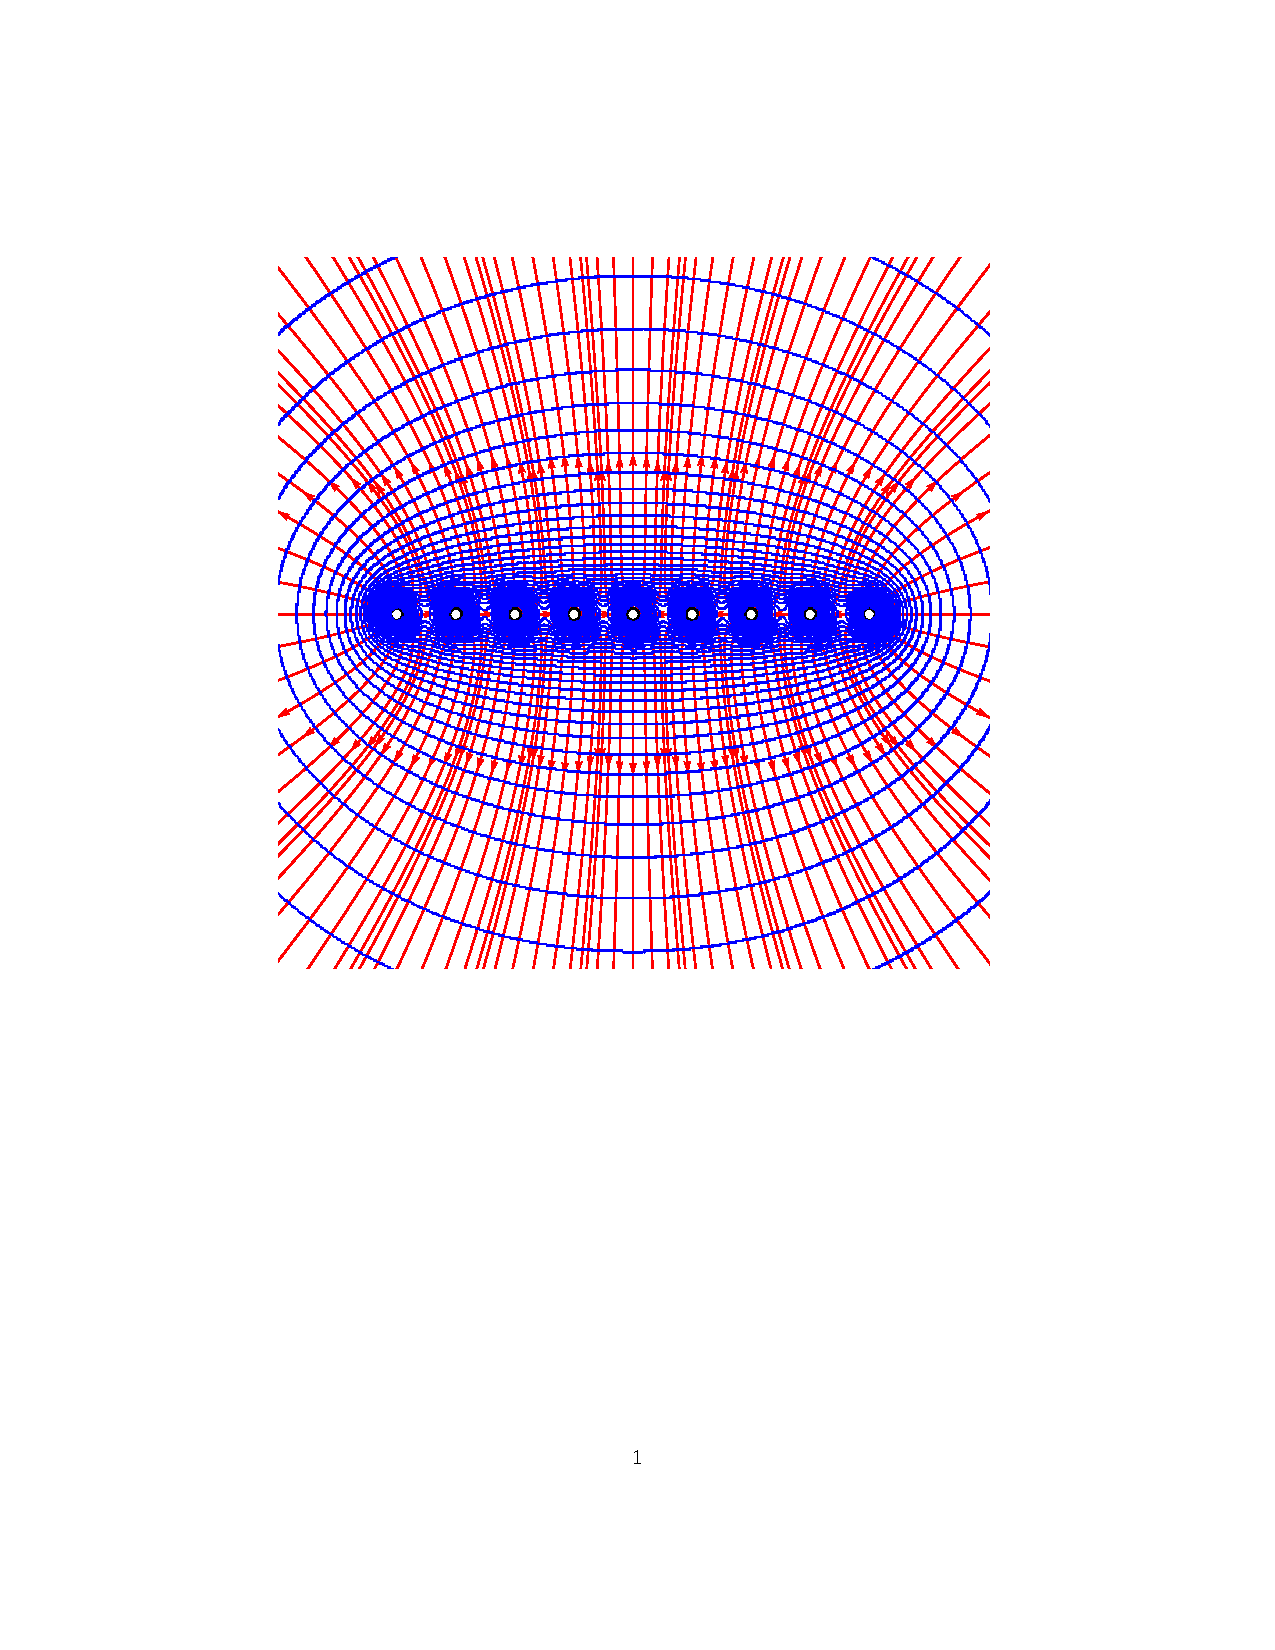
\includegraphics[width=\linewidth ,trim={6cm 14cm 6cm 7cm},clip]{Efield_graph_eq.pdf}
  \caption{Superposition of multiple positive point charges in a row}
  \label{fig:marginfig}
\end{marginfigure}
  Consider the situation of a uniform field, like that between two infinitely large charged plates.
  $$\Delta V=-\sum_A^B \overrightarrow{E}\cdot \Delta \overrightarrow{s}=-E\sum_A^B \Delta S=-E (B-A)=-ED$$
  In this case the potential varies linearly.  This is known as Ed's law.  It is generally applicable at a scale where the field is constant.
  \subsection{Point Charge}
  \begin{marginfigure}[0pt]%
  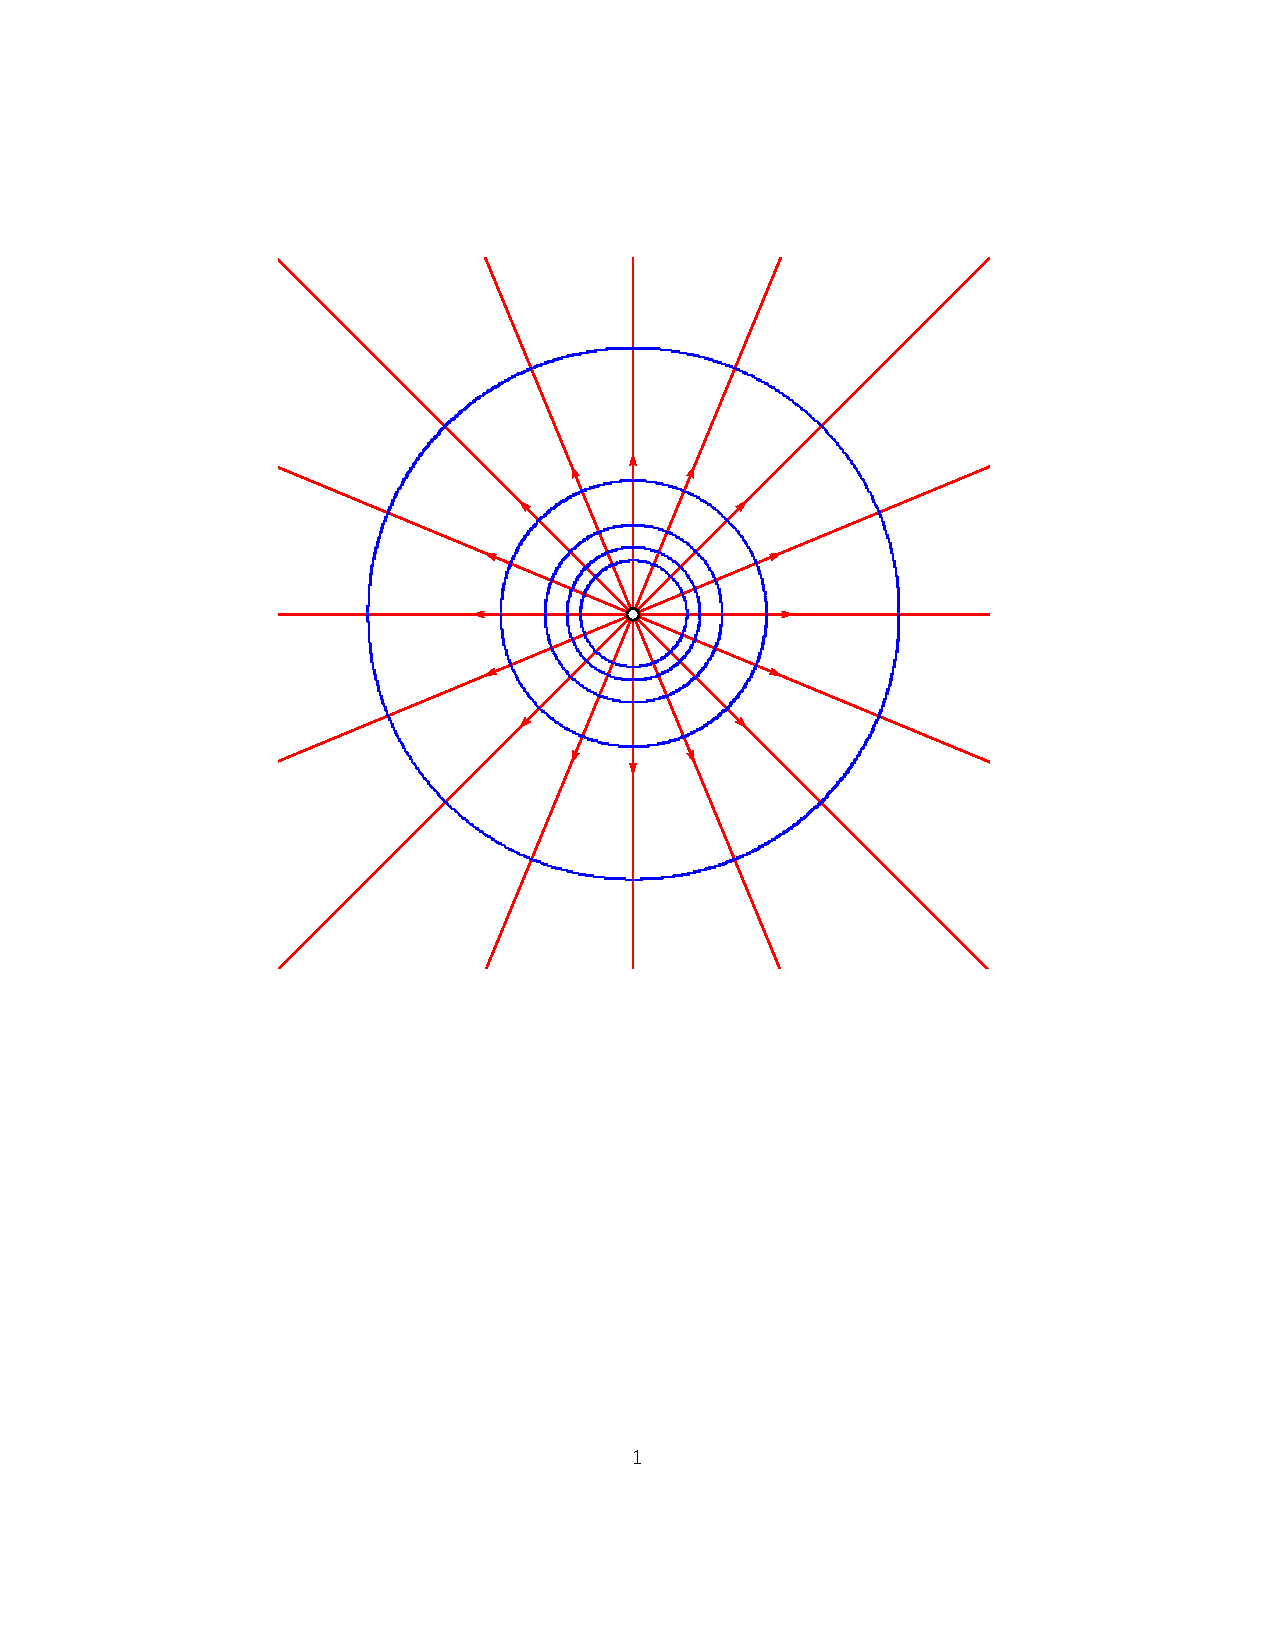
\includegraphics[width=\linewidth ,trim={7cm 14cm 7cm 7cm},clip]{Efield_graph3.pdf}
  \caption{Single positive charge with equipotential lines}
  \label{fig:marginfig}
\end{marginfigure}
  The potential around a point charge has the familiar $\frac{1}{r}$ dependence.
$$V=k_e\frac{q}{r} $$

\begin{marginfigure}[0pt]%
  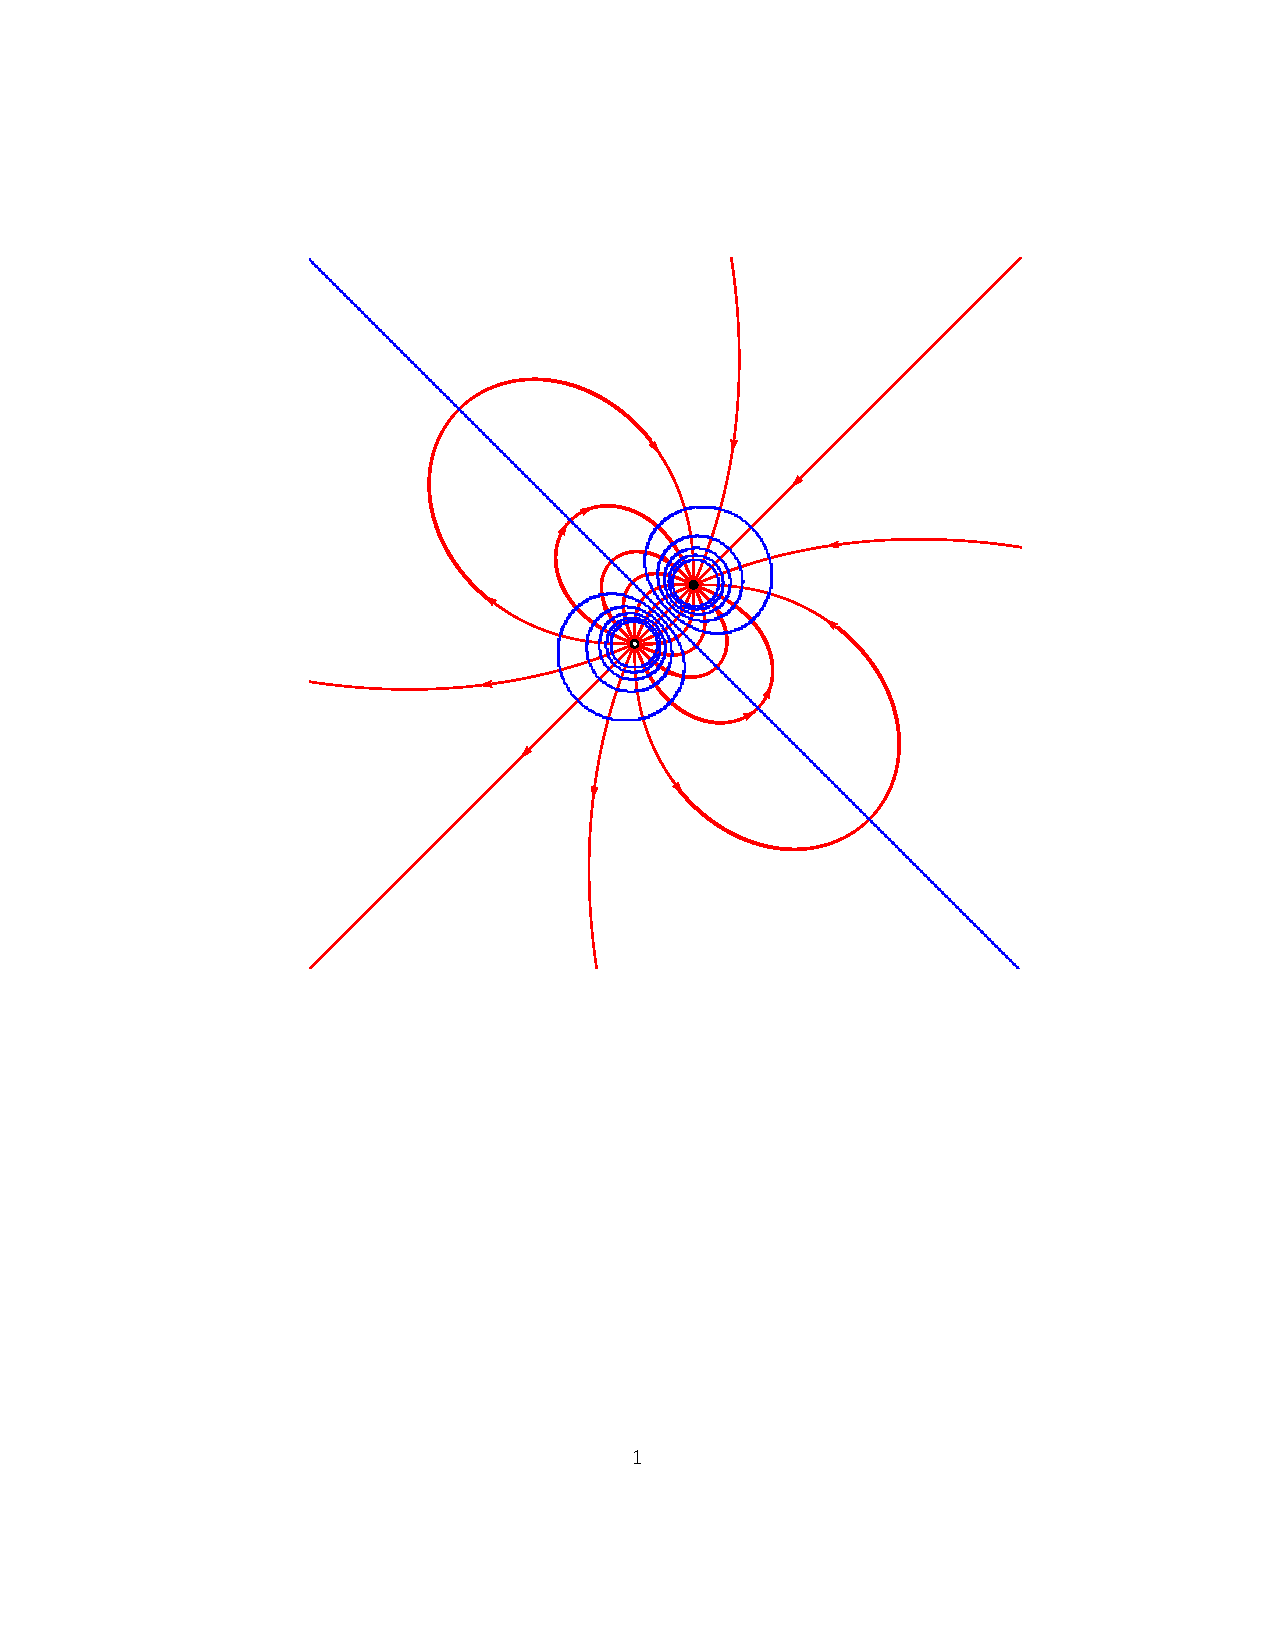
\includegraphics[width=\linewidth ,trim={7cm 14cm 7cm 7cm},clip]{dipole_graph_eq.pdf}
  \caption{Dipole field with equipotential lines}
  \label{fig:marginfig}
\end{marginfigure}

\subsection{Superposition of Point Charges}
$$V=k_e\sum_{i=1}^{N} \frac{q_i}{r_i} $$

%\subsection{Continuous Distribution}
%$$V=k_e\int \frac{dq}{r}$$



   \subsection{Vector Field, Scalar Field and Gradient}
     $$\overrightarrow{E}=-\lim_{\Delta \rightarrow 0}\left[\begin{array}{c} \nicefrac{\Delta V}{\Delta x} \\ \nicefrac{\Delta V}{\Delta y} \\ \nicefrac{\Delta V}{\Delta z}\end{array}\right]=-\lim_{\Delta \rightarrow 0}\left[\begin{array}{c} \nicefrac{\Delta }{\Delta x} \\ \nicefrac{\Delta }{\Delta y} \\ \nicefrac{\Delta }{\Delta z}\end{array}\right]V=-\nabla{V}$$
   \subsection{Equipotential Surfaces}
   Equipotential lines, or surfaces in 3-D, are equivalent to contour lines on a topographical map showing lines of equal elevation.
   \begin{itemize}
   \item An equipotential surface is any surface consisting of a continuous distribution of points held at the same electric potential.
   \item Electric field lines intersect equipotential lines at right angles.  They are perpendicular.
   \item Connected conductors share the same potential value.
   \end{itemize} 

%\chapter{Circuits \& Current}

\textit{Where there is power, there is resistance.}\\
\noindent\textbf{-   Michel Foucault}

\vspace{1cm}

\begin{marginfigure}%
  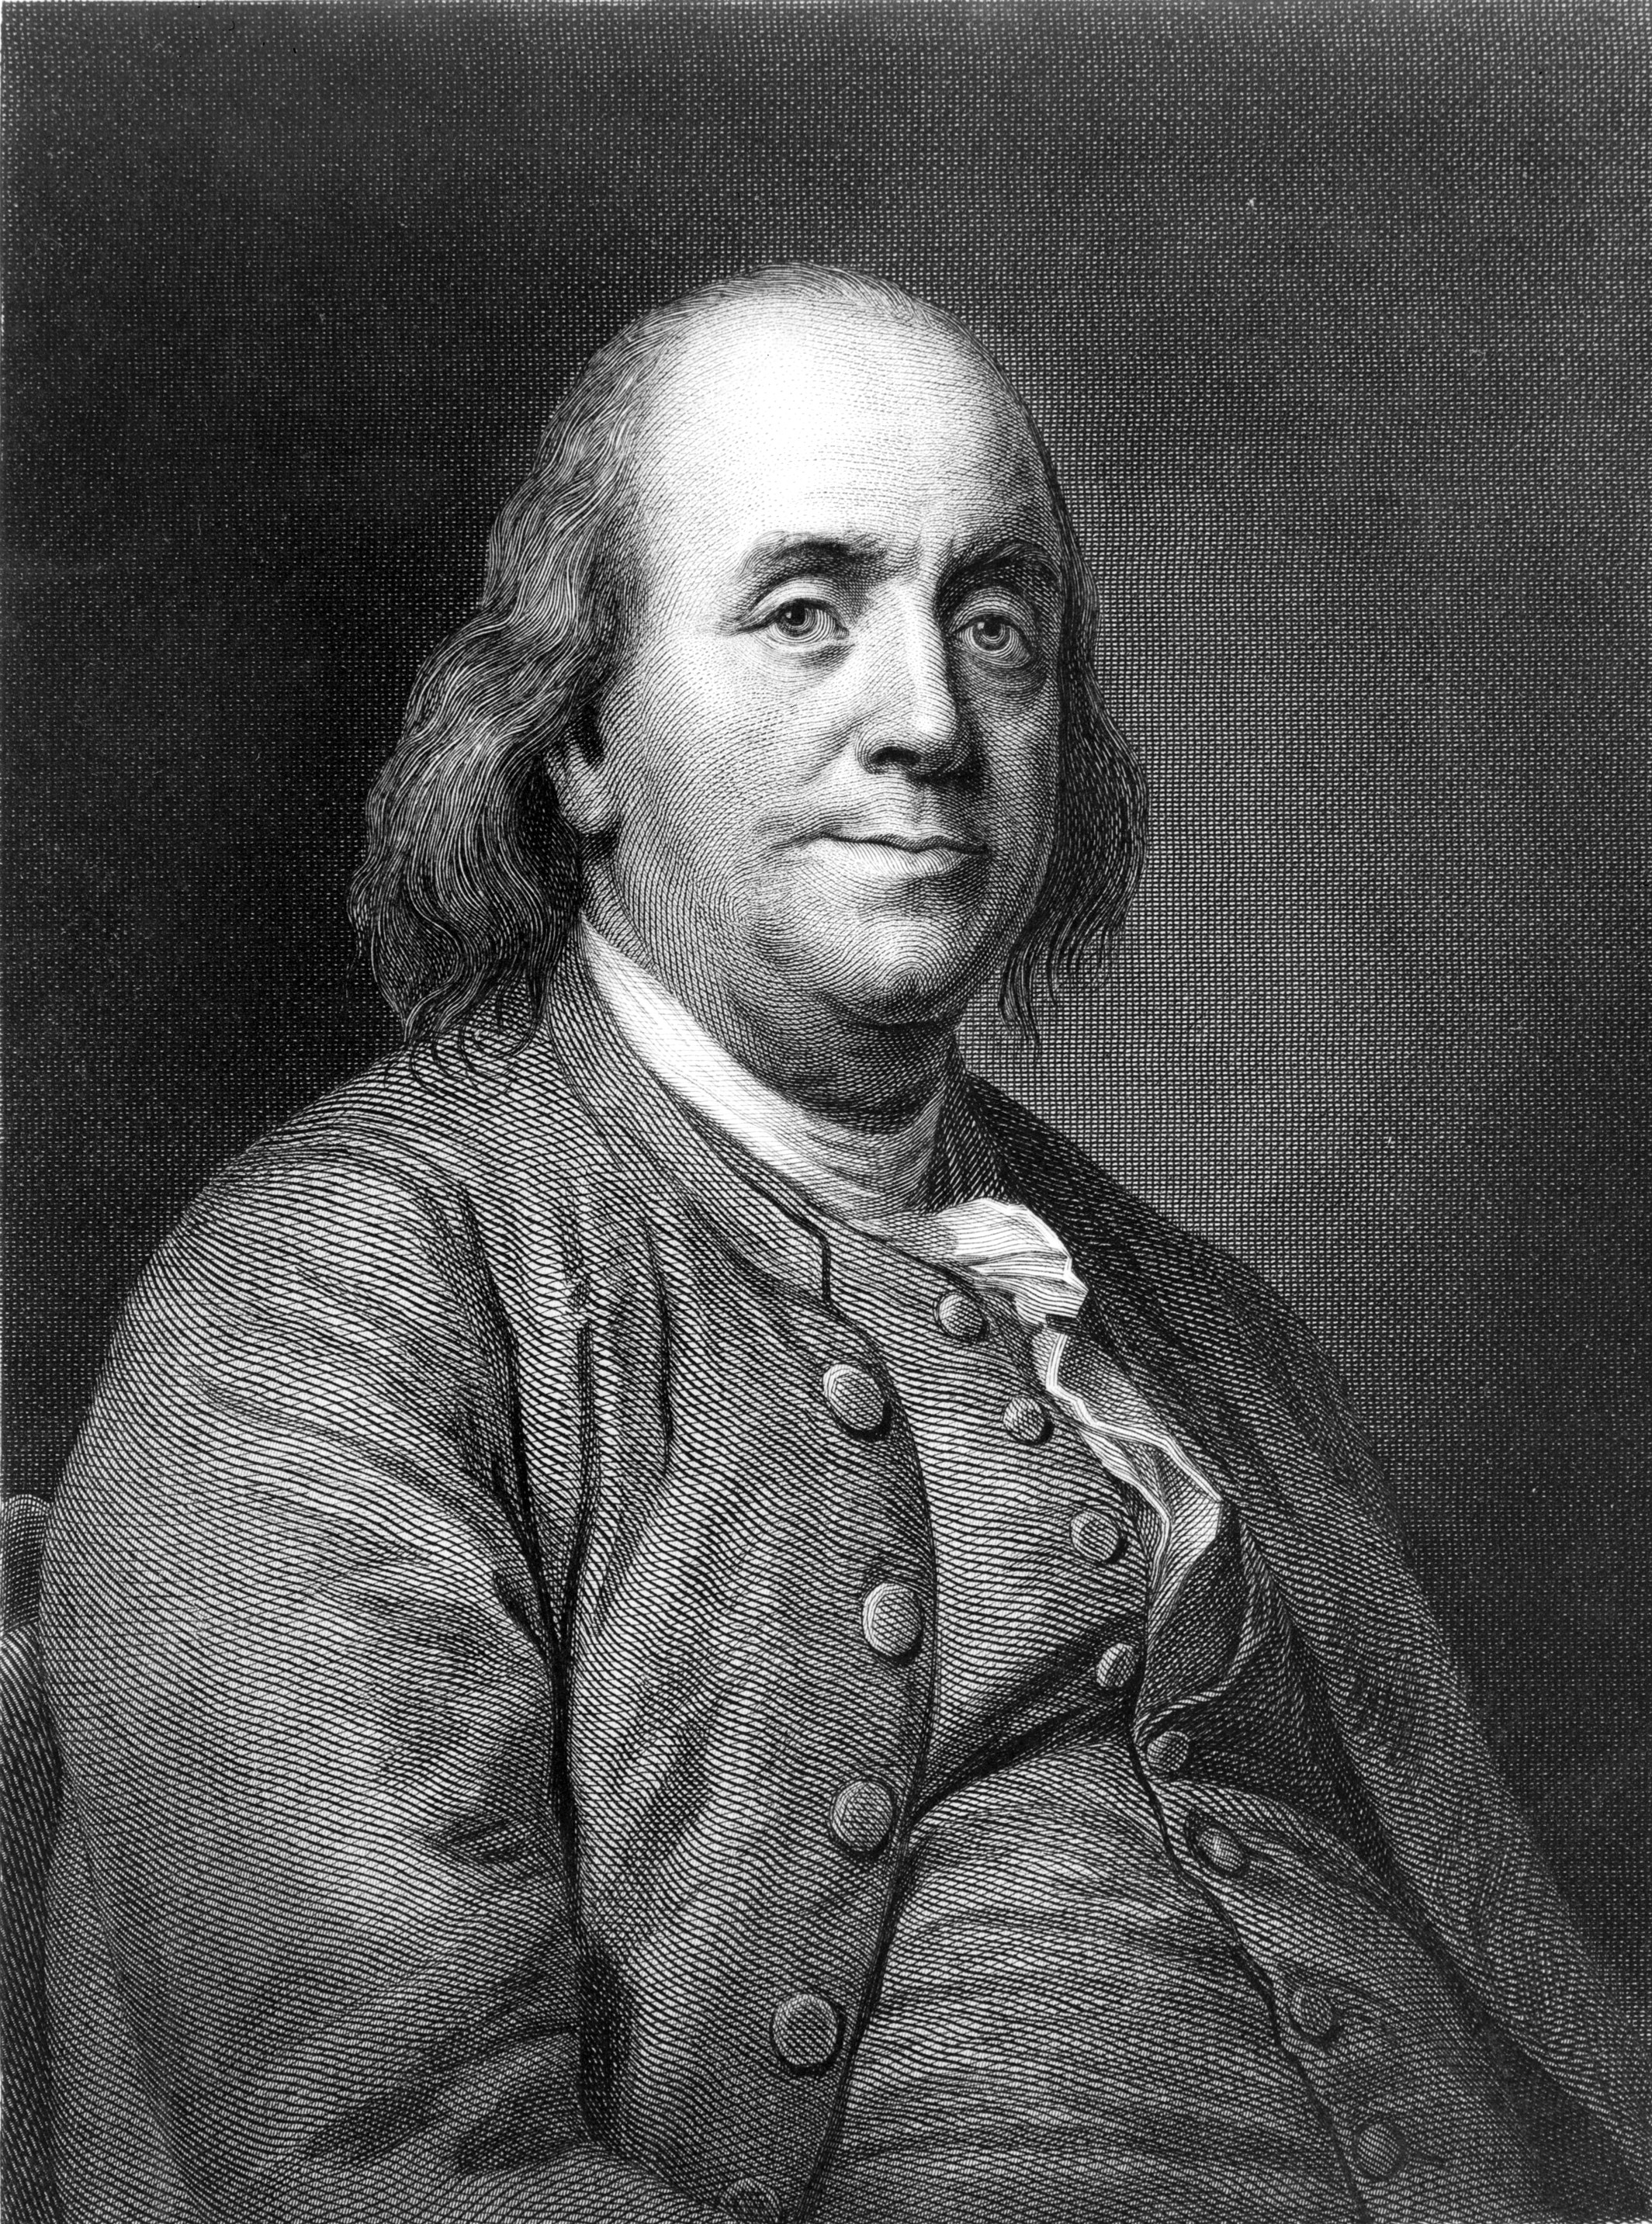
\includegraphics[width=\linewidth]{ben.jpg}
  \caption{Benjamin Franklin $\heartsuit$'s electricity}
  \label{fig:marginfig}
\end{marginfigure}

\section{Capacitance}
A capacitor holds a charge $+Q$ and $-Q$ on two plates at a given separation.   There is a voltage difference between the two plates $V$.
Capacitance is the ability of a body to store an electrical charge. A material with a large capacitance holds more electric charge at a given voltage, than one with low capacitance.  It is defined as the charge stored per volt.
$$C\equiv\frac{Q}{V}$$
The unit of capacitance is the farad.
$$1\ \text{Farad}=\frac{\text{Coulomb}}{\text{Volt}}$$
Consider the capacitor holding charges $+Q$ and $-Q$ on two plates.  Each has an area $A$ and they are separated by a distance $d$.  The constant electric field $E$ and and voltage difference $V$ are given as follows. 
$$E=\frac{\sigma}{\epsilon_0}=\frac{Q}{A\epsilon_0} \hspace{2cm} V=Ed$$
In this context the capacitance may be written in terms of the plate area and the separation distance.  
$$C=\frac{\epsilon_0A}{d}$$
In other words, the capacitance is strictly a feature of the structure of the capacitor and not a function of the particular voltage it is held at or how much charge is on it for the given conditions.

\newpage
\begin{marginfigure}%
  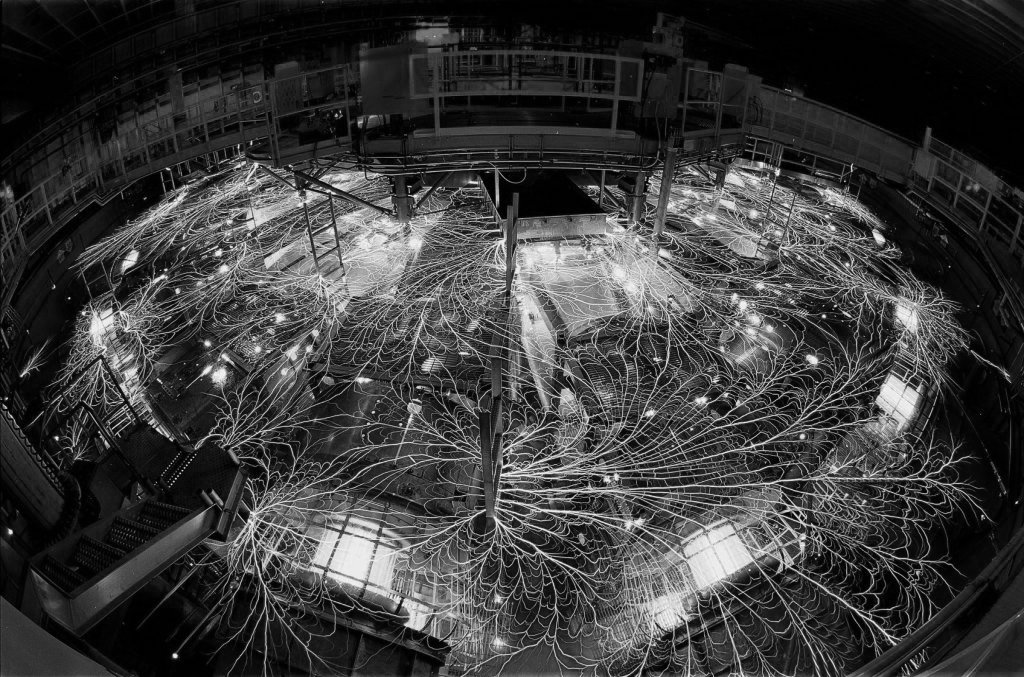
\includegraphics[width=\linewidth]{z-machine.jpg}
  \caption{The Z machine}
  \label{fig:marginfig}
\end{marginfigure}

\marginnote[30pt]{For a few billionths of a second the Z machine uses 80 times the entire world's electrical power output.}
\section{Circuit Combinations}
\subsection{Parallel}
Since the electrostatic force is conservative the voltage drop between two points should be independent of path.  Therefore the voltage drop across parallel capacitors should be equal.
$$V=V_1=V_2$$
In addition collapsing parallel capacitors into a single equivalent capacitor would have the charges add.
$$Q_{eq}=Q_1+Q_2$$
Substituting for each $Q$ using $Q=CV$ yields the next equation.
$$ C_{eq} V=C_1 V_1+C_2 V_2$$
Cancelling each of the equivalent voltages gives the following capacitance addition rule for parallel capacitors.
$$C_{eq}=C_1+C_2$$
$$\begin{circuitikz} 
\draw
(0,0) to[battery] (2,0) -- (2,2)
      to[capacitor, l=$C_1$] (0,2) -- (0,0);
      \draw (2,2) -- (2,4) to[capacitor, l=$C_2$] (0,4) -- (0,2);
\end{circuitikz}
\hspace{1cm} \text{equivalent to} \hspace{1cm} 
\begin{circuitikz} 
\draw
(0,0) to[battery] (2,0) -- (2,2)
      to[capacitor, l=$C_{eq}$] (0,2) -- (0,0);
\end{circuitikz}$$

\subsection{Series}
When capacitors are in series the voltages add to the total voltage of the circuit path.
$$V=V_1+V_2$$
The charges $Q_1$ and $Q_2$ are equal.  This is apparent when considering the floating circuit element shared by the two capacitors but completely isolated from the rest of the circuit.  Before the voltage is applied the charge in it is zero.  Once the voltage of the battery is applied the charge segregates, $+Q$ to one side and $-Q$ to the other side, conserving the total charge of zero.  Therefore the charge on the equivalent capacitor is equal to that on each of the series capacitors.
$$Q_{eq}=Q_1=Q_2$$
Starting with the voltage addition equation and substituting $V=\frac{Q}{C}$ for each component yields the following.
$$\frac{Q_{eq}}{C_{eq}}=\frac{Q_1}{C_1}+\frac{Q_2}{C_2}$$
Finally, cancelling the equal charge factors gives the equivalent capacitance for series capacitors.
$$\frac{1}{C_{eq}}=\frac{1}{C_1}+\frac{1}{C_2}$$
$$\begin{circuitikz} 
\draw
(0,0) to[battery] (4,0) -- (4,2)
      to[capacitor, l=$C_1$] (2,2) to[capacitor, l=$C_2$] (0,2) -- (0,0);
\end{circuitikz}
\hspace{1cm} \text{equivalent to} \hspace{1cm} 
\begin{circuitikz} 
\draw
(0,0) to[battery] (2,0) -- (2,2)
      to[capacitor, l=$C_{eq}$] (0,2) -- (0,0);
\end{circuitikz}$$

 
 \section{Dielectrics}
 A dielectric is a non-conductive material that increases the capacitance when placed between the two plates of a capacitor.
 $$C=\kappa C_0$$
 In such materials the $\epsilon$ replaces $\epsilon_0$.  
 $$\epsilon>\epsilon_0$$
 

\section{Energy Storage}
In order to determine the energy stored in a charged capacitor consider the small amount of work $w$ associated with adding a small amount of charge $\Delta q$ to a capacitor.
$$w=V \Delta q= \frac{q}{C}\  \Delta q$$
As more charge is added to the capacitor the voltage in the capacitor increases so the next small bit of charge requires more work to add than the previous.
$$W=\text{Area}(V(q))$$
$$PE=\frac{Q^2}{2C}=\frac{QV}{2}=\frac{CV^2}{2}$$

 \newpage
 
\section{Current}
\marginnote[0pt]{
$$1 \ \text{Ampere}=\frac{1\ \text{Coulomb}}{1\ \text{second}}$$
}
Electric current is the flow of charge.  It is the time rate of change of charge and is expressed in the unit of the ampere.
$$I \equiv \lim_{\Delta \rightarrow 0}\frac{\Delta Q}{\Delta t} \hspace{2cm} Q=\text{Area(I(t))}$$


Imagine setting up a toll both where the amount of charge flowing through the gate is counted per unit time.  This is current.
\subsection{Charge Carrier}
\marginnote[0pt]{
\begin{itemize}
\item n (carrier density)
\item q (carrier charge)
\item v (carrier velocity)
\item A (cross sectional area)
\end{itemize}
}
In electric circuits this charge is often carried by moving electrons in a wire. It can also be carried by ions in an electrolyte, or by both ions and electrons such as in a plasma.  The mobile charged body is known as the charge carrier.  The current can be determined by the number of charge carriers $N$ multiplied by the carrier charge $q$ per unit time $\Delta t$.
$$I=\frac{\Delta Q}{\Delta t}=\frac{N q}{\Delta t}$$
This can be expressed in terms of the the carrier density $n$.  This is the number of charge carriers per unit volume.
$$I=\frac{\Delta Q}{\Delta t}=\frac{n q}{\Delta t}V=nq\frac{\Delta x}{\Delta t}A=nqvA$$


\subsection{Current Density}
Current density $J$ is defined as the current passing through a cross-sectional area $A$.
$$J \equiv \frac{I}{A}=nqv$$

\section{Resistance \& Ohm's Law}
\marginnote[0pt]{
\begin{itemize}
\item $\sigma$ (conductivity)
\item $\rho$ (resistivity)
\item $l$ (length)
\item $R$ (resistance)
\end{itemize}
}
In an Ohmic material the current density is proportional to the electric field in the conductor.  The constant of proportionality $\sigma$ is known as the passivity.  
$$J=\sigma E$$
Starting fwith the above equation substitute the definition of current density and $E=\frac{V}{l}$ where $l$ is the length of the circuit element.
$$J=\frac{I}{A}=\sigma E=\sigma \frac{V}{l}$$
\marginnote[0pt]{
$$1\ \Omega=1 \ \text{Ohm}=\frac{1\ \text{Volt}}{1\ \text{Ampere}}$$
}
In circuits consisting of Ohmic materials the ratio between the voltage and the current is defined as the resistance $R$.
$$R\equiv \frac{V}{I}$$
$R$ may be expressed in terms of $\sigma$, $l$ and $A$ or the resistivity $\rho=\frac{1}{\sigma}$, the reciprocal of the passivity.
$$R=\frac{l}{\sigma A}=\rho\frac{l}{A}$$
\marginnote[-60pt]{Ohm's law is typically written as follows
$$V=IR$$}

\begin{margintable}[0pt]\index{typefaces!sizes}
  \footnotesize%
  \begin{center}
    \begin{tabular}{lc}
      \toprule
     Material & Resistivity ($\Omega\cdot \text{m}$) \\
      \midrule
     Copper     & 1.7$\times10^{-8}$  \\
    Aluminum      & 2.7$\times10^{-8}$  \\
    Tungsten (20 C)     & 5.6$\times10^{-8}$  \\
    Tungsten (1500 C)    & 5.0$\times10^{-7}$  \\
    Iron    & 9.7$\times10^{-8}$ \\
    Seawater      & 2.2$\times10^{-1}$  \\
    Blood     & 1.6  \\
    Muscle   & 1.3$\times10^{1}$  \\
    Fat      & 2.5$\times10^{1}$  \\
    Pure Water     & 2.4$\times10^{5}$  \\
    Cell Membrane     & 3.6$\times10^{7}$  \\
      \bottomrule
    \end{tabular}
  \end{center}
  \caption{A list of resistivities}
  \label{tab:font-sizes}
\end{margintable}


\section{Power}
$$P=IV$$
$$P=I^2R=\frac{V^2}{R}$$

\section{Resistors in Circuits}
\subsection{Series}
$$V=IR_1+IR_2=I(R_1+R_2)$$
$$V=IR_{eq} \hspace{2cm} R_{eq}=R_1+R_2$$

The current is the same in each resistor because any charge that flows through $R_1$ must also flow through $R_2$.

$$\begin{circuitikz} 
\draw
(0,0) to[battery] (4,0) -- (4,2)
      to[resistor, l=$R_2$] (2,2) to[resistor, l=$R_1$] (0,2) -- (0,0);
\end{circuitikz}
\hspace{1cm} \text{equivalent to} \hspace{1cm} 
\begin{circuitikz} 
\draw
(0,0) to[battery] (2,0) -- (2,2)
      to[resistor, l=$R_{eq}$] (0,2) -- (0,0);
\end{circuitikz}$$

\subsubsection{General}
$$R_{eq}=R_1+R_2+R_3 +\cdots$$

\subsection{Parallel}
The potential drop across parallel resistors is equal due to path independence of the potential function.  Additionally the total current going through each branch is conserved.
$$V=I_1R_1=I_2R_2$$
$$I=I_1+I_2$$
$$I=\frac{V}{R_1}+\frac{V}{R_2}=V\left(\frac{1}{R_1}+\frac{V}{R_1}\right)$$
$$I=\frac{V}{R_{eq}}$$
$$\frac{1}{R_{eq}}=\frac{1}{R_{1}}+\frac{1}{R_{2}}$$

$$\begin{circuitikz} 
\draw
(0,0) to[battery] (2,0) -- (2,2)
      to[resistor, l=$R_1$] (0,2) -- (0,0);
      \draw (2,2) -- (2,4) to[resistor, l=$R_2$] (0,4) -- (0,2);
\end{circuitikz}
\hspace{1cm} \text{equivalent to} \hspace{1cm} 
\begin{circuitikz} 
\draw
(0,0) to[battery] (2,0) -- (2,2)
      to[resistor, l=$R_{eq}$] (0,2) -- (0,0);
\end{circuitikz}$$
\subsubsection{General}
$$\frac{1}{R_{eq}}=\frac{1}{R_{1}}+\frac{1}{R_{2}}+\frac{1}{R_{3}}+\cdots$$

\section{Kirchoff's Rules}
\begin{itemize}
\item The sum of the currents entering a junction must be equal to the sum of the currents leaving that junction.
\item The algebraic sum of the changes in potential across all elements around any closed circuit must be zero.
\end{itemize}

\section{RC Circuits}
\marginnote[0pt]{Consider an uncharged capacitor in series with a resistor and a battery.  Initially there is no charge on it so there is no voltage drop across it.  Once the circuit is closed and the current begins to flow it begins to accumulate charge.  As it charges the rate of charging slows exponentially and approaches a maximum value asymptotically.}
$$\begin{circuitikz} 
\draw
(0,0) to[battery] (4,0) to[closing switch] (4,2)
      to[resistor, l=$R$] (2,2) to[capacitor, l=$C$] (0,2) -- (0,0);
\end{circuitikz}
$$

%$$V=V_R+V_C$$
%$$V=IR+\frac{q}{C}$$
%$$\frac{V}{R}=\frac{dq}{dt}+\frac{q}{RC}$$
%$$\int \frac{-dt}{RC}=\int \frac{dq}{q-CV}$$
\marginnote[50pt]{Consider an charged capacitor in series with a resistor and no battery.  Initially there is maximal charge on it so there maximal voltage drop across it.  Once the circuit is closed charge begins to flow of the capacitor.  As it discharges the rate slows exponentially and approaches a zero asymptotically.}
\subsection{Charging a Capacitor}
$$q(t)=CV(1-e^{-\frac{t}{RC}})=Q(1-e^{-\frac{t}{RC}})$$
$$I(t)=\frac{V}{R}e^{-\frac{t}{RC}}$$
\subsection{Discharging a Capacitor}
$$q(t)=Qe^{-\frac{t}{RC}}$$
$$I(t)=I_0e^{-\frac{t}{RC}}$$


%\chapter{Magnetism}

\textit{What magnetism is, no-one knows. We can only think of it as a peculiar condition created in space by the motion of electricity.}\\
\noindent\textbf{-   Sydney Evershed}

\vspace{1cm}


\begin{marginfigure}%
  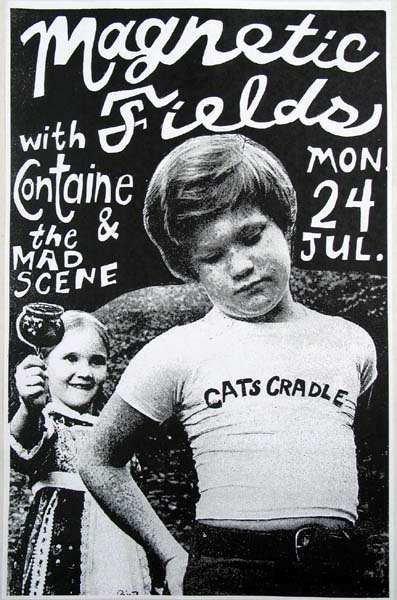
\includegraphics[width=\linewidth]{mag_fields.jpg}
  \caption{Magnetic Fields concert poster}
  \label{fig:marginfig}
\end{marginfigure}

Magnetism is the phenomenon of current interactions.  A current moving through space applies a force to other currents around it.  The story of magnetism is one of the deeper mysteries in physics.  As in electrostatics, physics uses the construct of the vector field to narrate the force interaction.

Currents generate magnetic fields in the space around them.  Currents also interact with fields in space.  This results in a magnetic force.  The story is therefore split into two parts.  How do currents generate fields in space?  How do currents interact with fields in space?  The present narrative addresses the second question first.


\section{Magnetic Force/Field}
Consider a a magnetic field in space $\overrightarrow{B}(\overrightarrow{r})$ and a particle with charge $q$ and velocity $\overrightarrow{v}$.   The resulting magnetic force is represented using the vector cross product.

$$\overrightarrow{F}_{B}=q\overrightarrow{v}\times \overrightarrow{B}$$
Remember the magnitude of the cross product is proportional to the $\sin$ of the angle between the field vector and the velocity vector.
$$F_{B}=qvB \sin \theta$$

\begin{marginfigure}[10pt]
 
\tdplotsetmaincoords{60}{110}
\begin{tikzpicture}[scale=1,tdplot_main_coords]
\coordinate (O) at (0,0,0);
\coordinate (P) at (1,2,3);

\draw[very thick,->] (0,0,0) -- (-2,2,0) node[anchor=south ]{$B$};
\draw[very thick,->] (0,0,0) -- (0,4,0) node[anchor=north west]{$v$};
\draw[very thick,->] (0,0,0) -- (0,0,3) node[anchor=south]{$F_{B}$};
\fill (0,0,0) circle(1mm) node[anchor=north east]{$q$};
%draw a vector from origin to point (P) 
\draw (-0.6,1.2,0) node[anchor=center,color=black]{$\theta$};


%draw projection on xy plane, and a connecting line
%syntax: \tdplotdrawarc[coordinate frame, draw options]{center point}{r}{angle}{label options}{label}
%\tdplotdrawarc{(O)}{0.2}{0}{\phivec}{anchor=north}{$\phi$}


%set the rotated coordinate system so the x'-y' plane lies within the
%"theta plane" of the main coordinate system
%syntax: \tdplotsetthetaplanecoords{\phi}
%\tdplotsetthetaplanecoords{\phivec}

%draw theta arc and label, using rotated coordinate system
%\tdplotdrawarc[tdplot_rotated_coords]{(0,0,0)}{0.5}{0}{\thetavec}{anchor=south west}{$\theta$}

\end{tikzpicture}

  \caption{Force of a moving charged particle in a magnetic field}
  \label{fig:marginfig}
\end{marginfigure}


\subsection{Unit}
The SI unit of magnetic field is the Tesla, named after Serbian-American mad scientist Nikola Tesla.
$$1 \ \text{Tesla}=\frac{1\ \text{Newton}}{1\ \text{Ampere} \cdot \text{meter}}$$

\newpage
\begin{marginfigure}%
  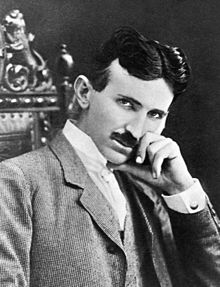
\includegraphics[width=\linewidth]{tesla.jpg}
  \caption{Handsome: Nikola Tesla}
  \label{fig:marginfig}
\end{marginfigure}


\subsection{No Work}
Since the magnetic force is always perpendicular to the velocity (displacement) no work is done by a static magnetic field on a moving particle.
$$W_B=\sum \overrightarrow{F}_B\cdot \ \Delta\overrightarrow{s}=\sum \overrightarrow{F}_B\cdot\overrightarrow{v}\ \Delta t=0$$
Fields may do work on magnetic dipoles, namely loops of current, but these are rigid bodies.  A constant magnetic field does not work on a single moving charged particle.
\section{Magnetic Force on a Straight Wire }
For $N$ charges particle in wire of length $L$ and cross-sectional area $A$, the total force on the wire is given as follows.

$$\overrightarrow{F}_{wire}=Nq\overrightarrow{v}\times \overrightarrow{B}= (nAL)q\overrightarrow{v}\times \overrightarrow{B}$$ 
Recall the expression for current as a charge rate of flux.  
$$I=nqvA=\overrightarrow J \cdot \overrightarrow A $$
In this way the force can be expressed in terms of the current and the length of the wire.  Since the force is a vector product each factor in the product must be a vector.  since the current is technically a scalar we vectorize the length in the notation.  Of course a length by itself is not a true vector but rather a pseudo-vector.  The sign which lifts the ambiguity for the direction of the $\overrightarrow{L}$ vector is borrowed from the sign of the scalar current $I$.
$$\overrightarrow{F}_{wire}=I\overrightarrow{L}\times\overrightarrow{B} $$


\begin{marginfigure}%
  
 \tikzset{->-/.style={decoration={
  markings,
  mark=at position #1 with {\arrow{latex}}},postaction={decorate}}}
  
\begin{tikzpicture}[scale=1]
\draw[very thick,->-=.5] (0,3) -- (0,0) node[midway, anchor=west]{$I$};

\draw[->] (-1,0.3)--(-0.2,0.3);
\draw[->] (-1,0.5)--(-0.2,0.5);
\draw[->] (-1,0.7)--(-0.2,0.7);
\draw[->] (-1,0.9)--(-0.2,0.9);
\draw (-1,0.6) node[anchor=east]{$B$};

\begin{scope}[scale={1}, shift={(0.4,0.6)}]
\draw (0,0) circle(1.8mm);
\fill (0,0) circle(0.3mm);
\draw (0.2,0) node[anchor=west]{$F$};
\end{scope}
\end{tikzpicture}


  \caption{Magnetic force on a current carrying wire }
  \label{fig:marginfig}
\end{marginfigure}



\section{General Wire}
For a general wire of any shape the approach is to break it up into small pieces of current carrying wire $\Delta\overrightarrow{s}$ and calculate the force $\Delta\overrightarrow{F}_{wire}$ on each piece.  We use the variable $i$ as an index for the pieces. 
$$\Delta\overrightarrow{F}_{i}=I\ \Delta\overrightarrow{s}_i\times\overrightarrow{B}(\overrightarrow{r}_i) $$
To calculate the total force a sum over the index $i$ is taken.  This add up all the little vector forces into a total force vector $\overrightarrow{F}_{wire}$.
$$\overrightarrow{F}_{wire}=\sum_i \Delta\overrightarrow{F}_{i}=\sum_i I\ \Delta\overrightarrow{s}_i\times\overrightarrow{B} (\overrightarrow{r}_i)$$
\newpage

\marginnote{One of the first drawings of a magnetic field, by Ren� Descartes, 1644. It illustrated his theory that magnetism was caused by the circulation of tiny helical particles, "threaded parts", through threaded pores in magnets.}

\begin{marginfigure}[20pt]%
  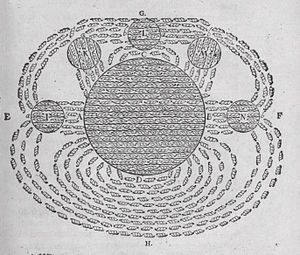
\includegraphics[width=\linewidth]{descartes_field.jpg}
  \caption{Descartes 1644 representation of the magnetic field}
  \label{fig:marginfig}
\end{marginfigure}

\subsection{Uniform Static Field: Path Independence}
A uniform and static magnetic field is constant over space and time.  $\overrightarrow{B} (\overrightarrow{r}_i)=\overrightarrow{B} $ so the summation is only on the path elements and dependent on spatial variation in the magnetic field. Such a field generates no net force.
$$\overrightarrow{F}_{wire}=I \left(\sum_a^b \ \Delta\overrightarrow{s} \right) \times\overrightarrow{B} =I\overrightarrow{s}_{ab}\times\overrightarrow{B} $$
 Such a field generates no net force.  This is because a loop has the same beginning point and end point.
$$\overrightarrow{F}_{wire}=I \left(\sum_a^a \ \Delta\overrightarrow{s} \right) \times\overrightarrow{B}=0 $$


\section{Torque on a Current Loop}
 
 \begin{marginfigure}[20pt]%

 
 \tikzset{->-/.style={decoration={
  markings,
  mark=at position #1 with {\arrow{latex}}},postaction={decorate}}}
  
\begin{tikzpicture}[scale=1]
\draw[very thick,->-=.5] (0,0) -- (2,0);
\draw[very thick,->-=.5] (2,0) -- (2,3)node[midway, anchor=west]{$I$};
\draw[very thick,->-=.5] (2,3) -- (0,3) ;
\draw[very thick,->-=.5] (0,3) -- (0,0);
\draw[->] (-1,0.3)--(-0.2,0.3);
\draw[->] (-1,0.5)--(-0.2,0.5);
\draw[->] (-1,0.7)--(-0.2,0.7);
\draw[->] (-1,0.9)--(-0.2,0.9);
\draw (-1,0.6) node[anchor=east]{$B$};

\begin{scope}[scale={1}, shift={(-0.4,2.4)}]
\draw (0,0) circle(1.8mm);
\fill (0,0) circle(0.3mm);
\draw (-0.2,0) node[anchor=east]{$F_1$};
\end{scope}

\begin{scope}[scale={1}, shift={(2.4,2.4)}]
\draw (0,0) circle(1.8mm);
\fill (0,0) circle(0.3mm);
\draw (0.2,0) node[anchor=west]{$F_2$};
\begin{scope}[scale={1}, rotate={(45)}]
\draw(-0.18,0) -- (0.18,0);
\draw(0,-0.18) -- (0,0.18);
\end{scope}
\end{scope}
\end{tikzpicture}

  \caption{Torque on a closed loop}
  \label{fig:marginfig}
\end{marginfigure}
While the total force is zero for a uniform magnetic field on a closed current loop there is a net torque on the loop.  Consider a rectangular loop of current with area $A$ and uniform magnetic field $B$.  The total torque is the product of the area and the magnetic field. 
$$ \tau=IAB$$
$$ \overrightarrow{\tau}=I\overrightarrow{A}\times \overrightarrow{B}$$
\subsection{Magnetic Moment}
The magnetic moment is defined as product of the current and the area.  Note that the current is a scalar and area is a vector.  Thus the magnetic moment is a vector quantity.
$$\overrightarrow{\mu}= I \overrightarrow{A}$$
The torque on the loop may be parameterized in terms of the magnetic moment.
$$\overrightarrow{\tau}=\overrightarrow{\mu}\times \overrightarrow{B}$$
\section{Homopolar Electric Motor}
The homopolar motor was the first electrical motor to be built. Its operation was demonstrated by Michael Faraday in 1821 at the Royal Institution in London.  It is driven by a Lorentz force.  A paper clip, AAA battery and permanent magnet constitute a homopolar motor.
\begin{marginfigure}[-180pt]%
  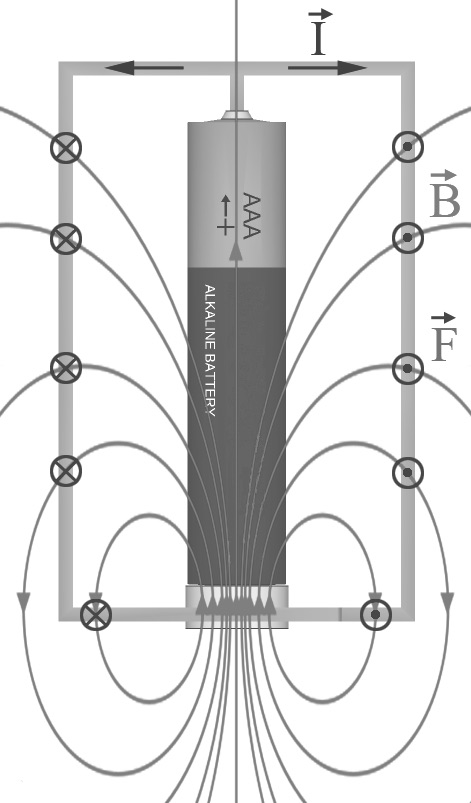
\includegraphics[width=\linewidth]{homopolar_motor.jpg}
  \caption{Simple homopolar motor}
  \label{fig:marginfig}
\end{marginfigure}


\newpage
\section{Circular Motion of a Charged Particle in a Uniform B Field}
\begin{marginfigure}[0pt]%
  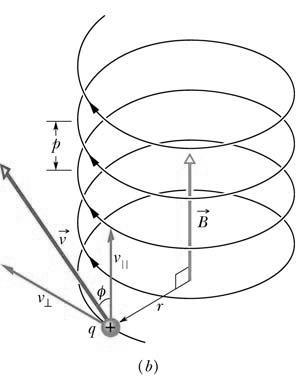
\includegraphics[width=\linewidth]{helix.jpg}
  \caption{Helical motion of a charged particle in a magnetic field}
  \label{fig:marginfig}
\end{marginfigure}
$$F_B=F_c$$
$$ qv_{\perp}B=\frac{mv_{\perp}^2}{r}$$
$$\frac{v_{\perp}}{r}=\omega=\frac{qB}{m}$$
\section{General Motion}
The total force on an electric field and magnetic field on a moving charged particle is known as the Lorentz force.
$$\overrightarrow{F}=q\overrightarrow{E}+q\overrightarrow{v}\times\overrightarrow{B}$$
\section{Velocity Selector}
For perpendicular electric and magnetic fields the Lorentz force will be zero on particle on a particle traveling with a perpendicular component of velocity equal to the ratio of electric field to magnetic field.
$$\overrightarrow{E}=E\hat{x} \hspace{1cm} \overrightarrow{B}=B\hat{y} \hspace{1cm} \overrightarrow{v}=v\hat{z}$$
$$\overrightarrow{F}=qE\hat{x}+qvB\hat{z}\times\hat{y}=q(E-vB)\hat{x}$$
$$v=\frac{E}{B}$$

\begin{marginfigure}
  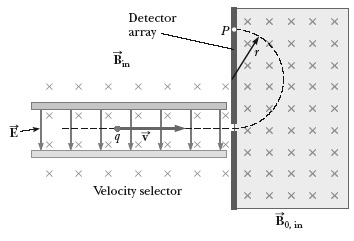
\includegraphics[width=\linewidth]{selector.jpg}
  \caption{Mass spectroscopy with a velocity selector and a detector plate in a constant magnetic field }
  \label{fig:marginfig}
\end{marginfigure}


\section{Mass Spectroscopy}
Mass spectroscopy leverages the physics of the velocity selector and circular motion in a magnetic field to precisely measure mass to charge ratio.  The radius of curvature of the particle is $r$.
$$r=\frac{mv}{qB}$$
Therefore measuring the electric field, magnetic field and radius of curvature would determine the mass to charge ratio of the particle.

$$\frac{m}{q}=\frac{rB}{v}=\frac{rB^2}{E}$$ 
\section{Sources of Magnetic Field}
Up until now there have only been description of currents interacting with existing magnetic fields.  The second half of the story of magnetism addresses how those fields are generated.

The general law for determining the magnetic field in space $\overrightarrow{B}(\overrightarrow{r})$ generated by a current through a general wire is complex and cumbersome.  We begin with a description of the little bit of magnetic field $ \Delta \overrightarrow{B}$ generated by a current $I$ traveling through a small length of wire $\overrightarrow{s}$.  The vector from the the section of wire to the point in space is $\overrightarrow{r}$.  This is known as the Biot-Savart law.
$$\text{Biot-Savart Law} \hspace{2cm} \Delta \overrightarrow{B}=k_m\frac{I\ \Delta\overrightarrow{s}\times \hat{r}}{r^2}$$
There is a constant of proportionality $k_m$ analogous to the $k_e$ for electric fields.  We may also parameterize this constant in terms of the magnetic permeability of free space $\mu_0$.
$$k_m=\frac{\mu_0}{4\pi} =10^{-7}\  \frac{\text{Tm}}{\text{A}}$$
$$\text{Magnetic Permeability of Free Space} \hspace{2cm} \mu_0=4\pi\times10^{-7}\  \frac{\text{Tm}}{\text{A}}$$
In order to get the magnetic field at a point in space all the  contributions from all the small bits of wire must be summed up.
$$\overrightarrow{B}=\sum \Delta \overrightarrow{B}= \frac{\mu_0I}{4\pi}\sum \frac{\Delta\overrightarrow{s}\times \hat{r}}{r^2}$$

\section{B Field Around an Infinitely Long Straight Wire}
Consider a long straight wire carrying a current $I$.  We cut cut the wire into little pieces of length $\Delta x$ each having an angle$\theta$ with the point in question a distance $a$ away from the wire.  The contribution of each segment of wire is given here.
$$\Delta B=\frac{\mu_0I}{4\pi}\frac{\Delta x\ \sin\theta}{r^2}$$
The contributions from all the pieces of wire gives a total magnetic field at the point in question proportional to one over the distance.
$$B=\frac{\mu_0I}{2\pi a}$$
\section{B Field Above a Current Loop}
The magnetic field a distance $x$ above a loop of current, with radius $R$, is derived as follows.
$$\Delta B=\frac{\mu_0I}{4\pi}\frac{|\Delta\overrightarrow{s}\times \hat{r}|}{r^2}=\frac{\mu_0I}{4\pi}\frac{\Delta s}{x^2+R^2}$$
The sum of all the components yields the following.
$$B=\frac{\mu_0IR^2}{2(x^2+R^2)^{3/2}}$$
In the limit of the distance much larger than the radius, $x>>R$, we get the following.
$$B=\frac{\mu_0IR^2}{2x^3}$$
\begin{marginfigure}
  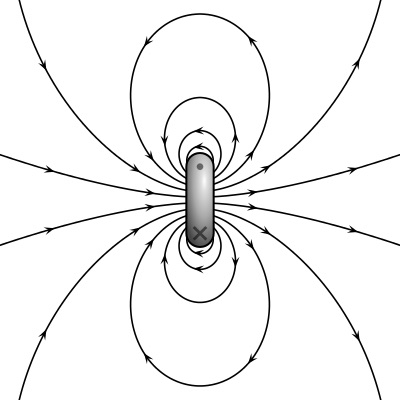
\includegraphics[width=\linewidth]{mag_dipole.jpg}
  \caption{Magnetic field around a loop of current}
  \label{fig:marginfig}
\end{marginfigure}
\section{Magnetic Force Between Two Parallel Wires}
Consider the force between two parallel wires.
$$\frac{F_1}{l}=\frac{\mu_0I_1I_2}{2\pi a}$$
This force is attractive if the the currents are in the same direction and repulsive if the wires are in opposite directions.

\section{Ampere's Law}
Ampere's law is the elegant representation describing the magnetic field around a current $I$.  We use an Amperian loop $s$ as a tool to determine the magnetic field 
$$\sum_{closed} \overrightarrow{B}\cdot \Delta\overrightarrow{s}=\mu_0I$$ 
The line integral of $\overrightarrow{B}\cdot \Delta\overrightarrow{s}$ around any closed path equals $\mu_0I$, where I is the total steady state current 
passing through any surface bounded by the closed path Amperian loop.
\subsection{Symmetric Path and Field}
If the field is uniform along the closed path then the summation reduces.
$$BS=\mu_0I$$ 
\section{B Field Inside a Solenoid}
A solenoid is a winding loop of current.  The magnetic field inside a solenoid maybe easily determined using Ampere's law using a rectangular loop of length $l$.
$$\sum_{closed} \overrightarrow{B}\cdot \Delta \overrightarrow{s}=Bl$$
$N$ is the number of winding turns through the loop.
$$Bl=\mu_0NI$$
It reduces to a linear dependence on the the density of turns per unit length $n$.
$$B=\mu_0nI$$

\section{Magnetic Flux}
Magnetic flux is defined as the total amount of magnetic field going through a surface.
$$\Phi_B=\sum \overrightarrow{B}\cdot d \overrightarrow{A}$$
The total magnetic flux going through a closed surface is zero.  This is known as Gauss's law for magnetism.
$$\sum_{closed} \overrightarrow{B}\cdot \Delta\overrightarrow{A}=0$$

\section{Displacement Current}
Displacement current is the effective current generated at a capacitor gap.  It is proportional to the time rate of change of electric flux.
$$I_d\equiv\epsilon_0\frac{d\Phi_E}{dt}$$
Since Ampere's law involves determining the current flux though the membrane bound by the Amperian loop is is possible to stretch the membrane so that it passed through the capacitor gap, where no actual current would pass through the membrane.  Therefore an increasing electric field must be considered equivalent to a real current.
$$\sum_{closed} \overrightarrow{B}\cdot \Delta \overrightarrow{s}=\mu_0(I+I_d)$$
An increasing electric field generates a magnetic field around it.  Therefore Ampere law requires a small addendum to include the displacement current.


\chapter{Induction}

\textit{I was at first almost frightened when I saw such mathematical force made to bear upon the subject, and then wondered to see that the subject stood it so well.}\\
\noindent\textbf{-   Michael Faraday}

\vspace{1cm}


\begin{marginfigure}%
  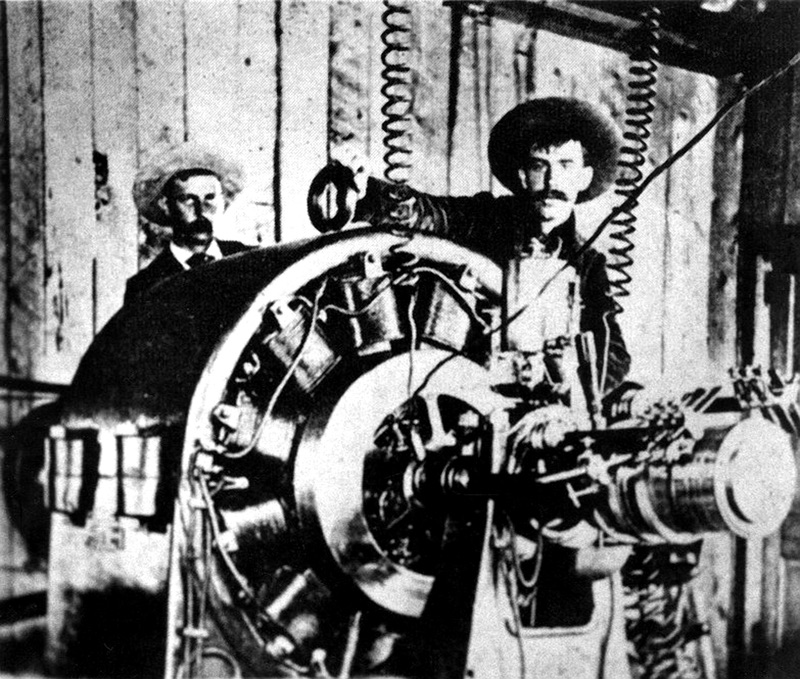
\includegraphics[width=\linewidth]{generator.jpg}
  \caption{Dudes posing with their Westinghouse alternator in 1891}
  \label{fig:marginfig}
\end{marginfigure}


\marginnote[20pt]{
\section{Magnetic Flux}
Magnetic flux $\Phi_B$ is the is the sum of magnetic field $\overrightarrow{B}$ passing through a surface area $\overrightarrow{A}$.
$$ \Phi_B=\sum\overrightarrow{B}\cdot \Delta\overrightarrow{A}$$ }


\begin{marginfigure}[20pt]%
  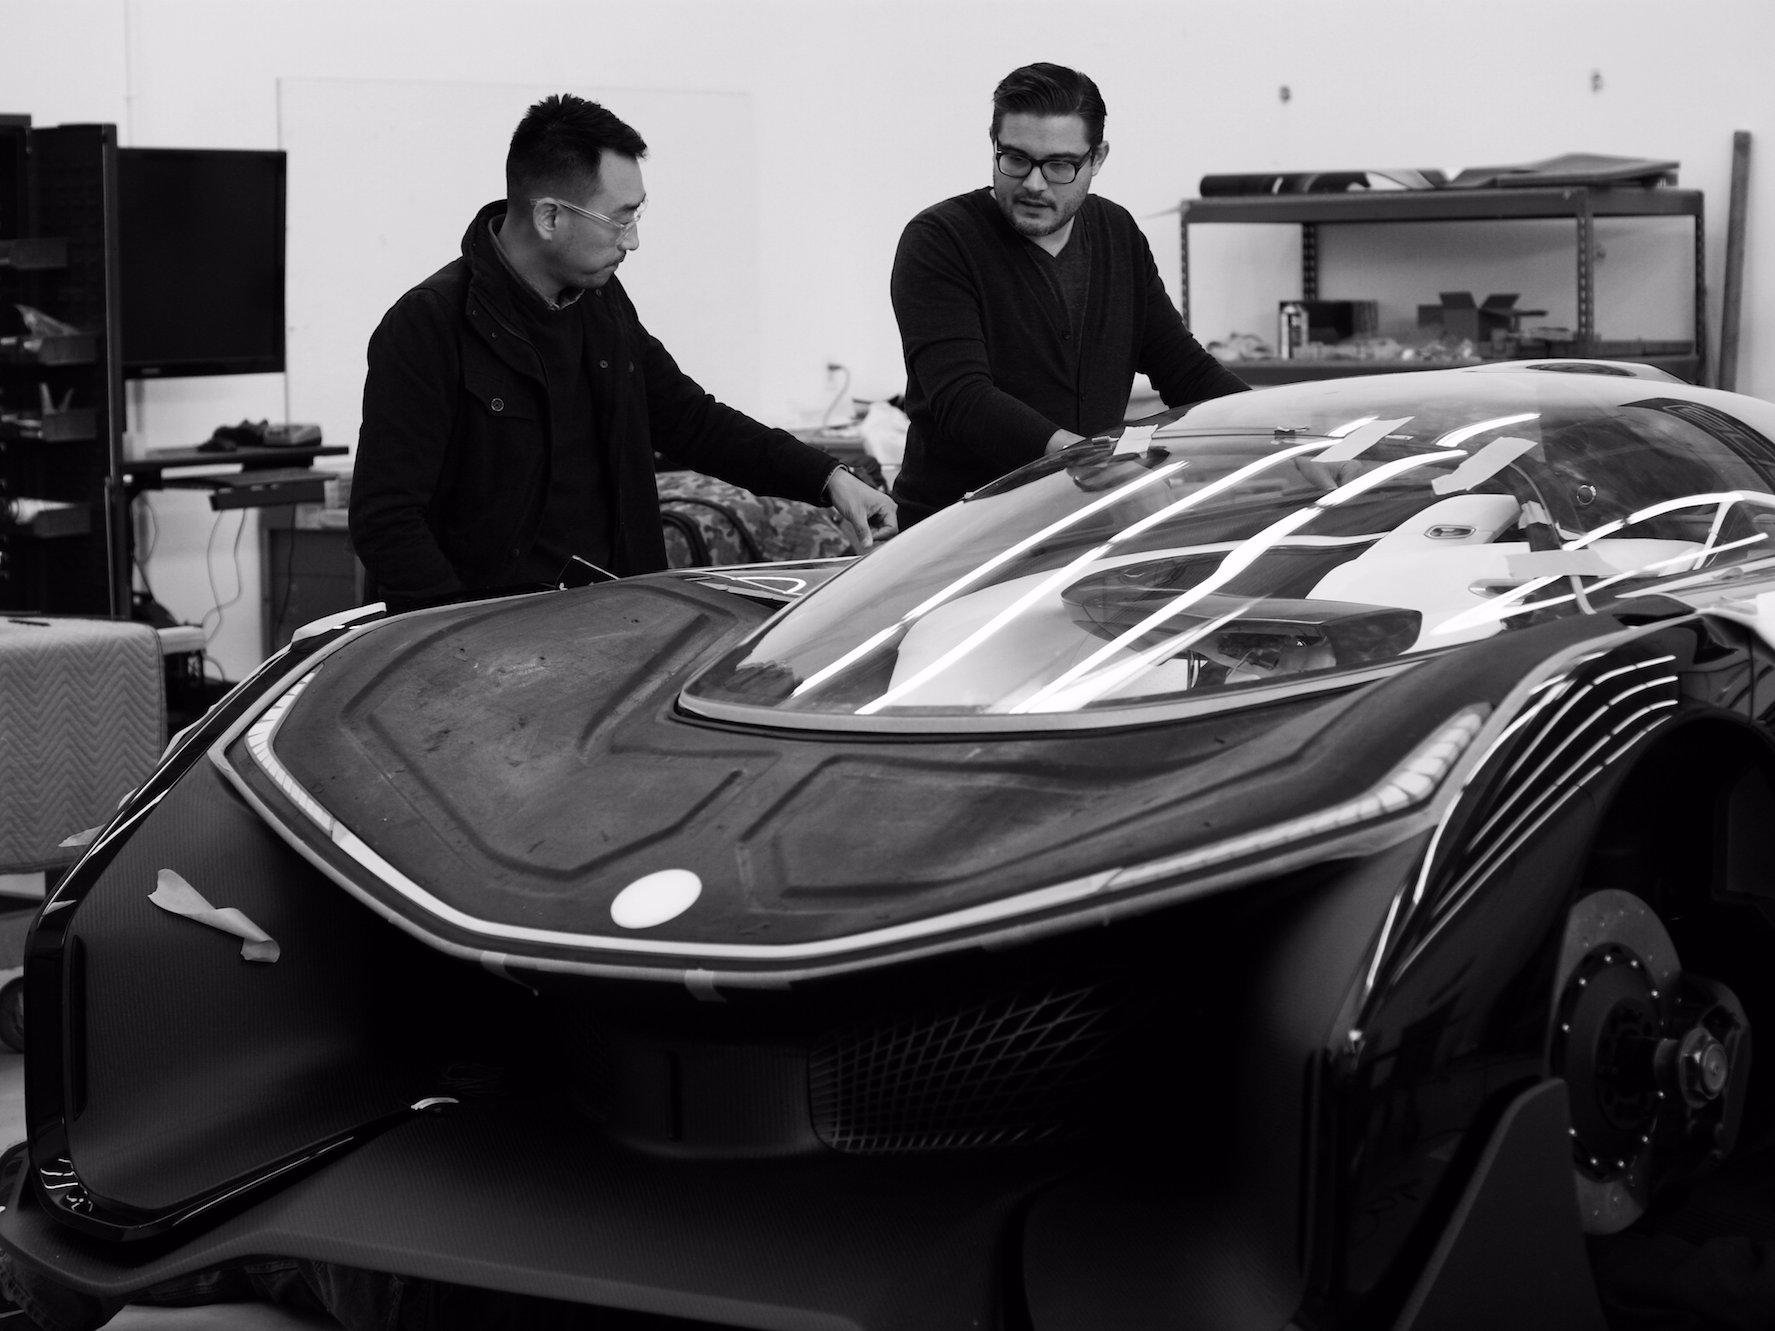
\includegraphics[width=\linewidth]{ffzero.jpg}
  \caption{\textit{Faraday Future} engineers prototyping the FFZERO in 2016  }
  \label{fig:marginfig}
\end{marginfigure}


\section{Electromotive Force}
Electromotive force, or emf, is denoted $\mathcal{E} $.  It is the voltage developed through a conducting circuit by a battery or dynamo.  It is not a force but an integral of the electric field over the current path.  It is similar to a voltage difference but may be non-zero over a closed path. 

\section{Motional Emf}
Consider a conducting bar of length $l$ moving perpendicularly through a magnetic field.  The charge carriers in the conductor undergo a magnetic force.  

$$\overrightarrow{F}_{B}=q\overrightarrow{v}\times \overrightarrow{B}$$

The conductor will polarize as the charge carriers move up until the point equilibrium is reached.  The effect is that an electric potential difference is maintained between the ends of a conductor moved perpendicularly through a magnetic field.  To determine the magnitude of this potential begin by equating the magnetic force and the electrostatic force.
$$F_E=F_B$$
$$qE=qvB \hspace{2cm} E=vB$$
Once the strength of the electric field is determined a potential difference is derived.
$$\Delta V=El=Blv$$

\newpage
\begin{marginfigure}[10pt]%
  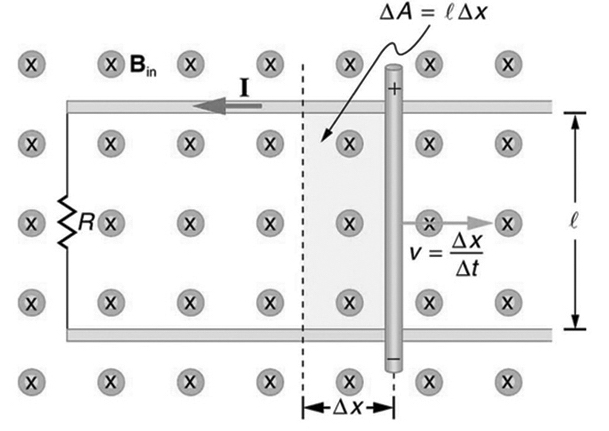
\includegraphics[width=\linewidth]{motional.jpeg}
  \caption{Motional emf}
  \label{fig:marginfig}
\end{marginfigure}
\noindent Now consider when the conducting bar is made part of a closed circuit with resistance $R$. In this case charge is free to flow through the circuit.  The bar is at position $x$.  The magnetic flux is determined as follows.
$$\Phi_B=Blx$$
The motional emf is determined.  
$$ \mathcal{E}=-\frac{d\Phi_B}{dt}=-Blv$$



\subsection{Power}
The power dissipated by the circuit is determined as follows.  Find the mechanical power.
$$P=Fv=IlBv=\frac{B^2l^2v^2}{R}$$
Find the electrical power. 
$$P=\frac{V^2}{R}=\frac{\mathcal{E}^2}{R}=\frac{B^2l^2v^2}{R}$$
Note their equivalence.


\section{Faraday's Law}
\begin{marginfigure}[150pt]%
  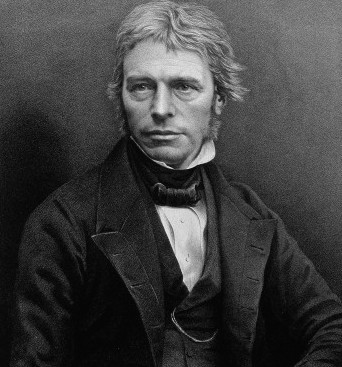
\includegraphics[width=\linewidth]{faraday.jpg}
  \caption{Michael Faraday}
  \label{fig:marginfig}
\end{marginfigure}

An emf is induced in a circuit by a changing magnetic field either by changing the area, relative orientation or strength of the magnetic field.  The induced emf is directly proportional to the time rate of change of the magnetic flux through the circuit.
$$ \mathcal{E}=-\frac{\Delta\Phi_B}{\Delta t} \hspace{2cm} \Phi_B=\sum\overrightarrow{B}\cdot \Delta\overrightarrow{A}$$
And for a circuit with $N$ coil loops.
$$ \mathcal{E}=-N\frac{\Delta\Phi_B}{\Delta t}$$



\section{Lenz's Law}
The induced emf produces a current which creates magnetic flux opposite the change of magnetic flux through the loop.\\ 

There are many ways to do this bookkeeping.  One way is to use a left hand rule.

\section{Induced Emf and Electric Field}
An electric field is generated in the conductor as a result of the changing magnetic flux.  In fact, an electric field is always generated by a changing magnetic flux, even in free space.
$$\sum_{\text{\tiny boundary}}\overrightarrow{E}\cdot \Delta\overrightarrow{s}=-\frac{\Delta\Phi_B}{\Delta t}$$


\section{Inductance}
\marginnote[-30pt]{
\subsection{Unit}
The unit for inductance is the Henry.  It is defined as the Volt second per Ampere.
$$1 \ \text{Henry}=\frac{1\ \text{Volt second}}{1\ \text{Ampere}}$$}
The term inductance was coined by Oliver Heaviside in 1886.  It is the property of an electrical conductor by which a change in current flowing through it induces an electromotive force in both the conductor itself (self-inductance) and in nearby conductors (mutual inductance).
$$ \mathcal{E}_L=-N\frac{\Delta\Phi_B}{\Delta t}=-L\frac{\Delta I}{\Delta t}$$
$$L=\frac{N\Phi_B}{I}$$



\section{RL Circuits}
\marginnote[0pt]{A simple RL circuit consists of a resistor and inductor in series with a battery.  The example circuit has a open switch that is closed at time $t=0$.  The resulting current approaches a constant value asymptotically.\\
Without the battery the circuit may be perturbed by giving the inductor a pulse of magnetic field.  In this case the current will decay exponentially.}
$$\begin{circuitikz} 
\draw
(0,0) to[battery] (4,0) to[closing switch] (4,2)
      to[resistor, l=$R$] (2,2) to[inductor, l=$L$] (0,2) -- (0,0);
\end{circuitikz}
$$
$$ \mathcal{E}=IR+L\frac{\Delta I}{\Delta t}$$
$$I(t)=\frac{\mathcal{E}}{R}\left(1-e^{-\frac{R}{L}t}\right)$$
%\vspace{1cm}

\section{LC Circuits}
\marginnote[0pt]{A simple LC circuit consists of a capacitor and inductor in series.  The example circuit begins with the capacitor charged and has a open switch that is closed at time $t=0$.  The resulting current is a sinusoidal oscillation.\\
Without the capacitor initially charged the circuit may be perturbed by giving the inductor a pulse of magnetic field.}
$$\begin{circuitikz} 
\draw
(0,0) -- (4,0) to[closing switch] (4,2)
      to[capacitor, l=$C$] (2,2) to[inductor, l=$L$] (0,2) -- (0,0);
\end{circuitikz}
$$
$$ 0=\frac{Q}{C}+L\frac{\Delta I}{\Delta t}$$
$$Q(t)=Q_0 \cos\left(\frac{t}{\sqrt{LC}}\right)$$
$$I(t)=-\frac{Q_0}{\sqrt{LC}} \sin\left(\frac{t}{\sqrt{LC}}\right)$$
%\vspace{1cm}
\section{Inductor Energy}
Consider the power dissipated in a RL circuit.
$$P=I \mathcal{E}=I^2R+LI\frac{\Delta I}{\Delta t}$$
The term representing the rate of change of energy stored in the magnetic field is shown below. 
$$\frac{\Delta U_B}{\Delta t}=LI\frac{\Delta I}{\Delta t}$$
The energy stored in the magnetic field is written as follows.
$$U_B=\frac{LI^2}{2}$$


\section{Maxwell's Equations}

\vspace{1cm}
\subsection{Gauss's Law}

$$\sum_{\text{\tiny boundary}}\overrightarrow{E}\cdot \Delta\overrightarrow{A}=\frac{q_{enc}}{\epsilon_0}$$

\vspace{1cm}
\subsection{Gauss's Law for Magnetism}

$$\sum_{\text{\tiny boundary}}\overrightarrow{B}\cdot \Delta\overrightarrow{A}=0$$

\vspace{1cm}
\subsection{Ampere-Maxwell Law}

$$\sum_{\text{\tiny boundary}}\overrightarrow{B}\cdot \Delta\overrightarrow{s}=\mu_0 I+\mu_0\epsilon_0\frac{\Delta\Phi_E}{\Delta t}$$

\vspace{1cm}
\subsection{Faraday's Law}

$$\sum_{\text{\tiny boundary}}\overrightarrow{E}\cdot \Delta\overrightarrow{s}=-\frac{\Delta\Phi_B}{\Delta t}$$


%\bibliography{sample-handout}
%\bibliographystyle{plainnat}


\printindex

\end{document}

